\documentclass[aps,prl,reprint,10pt,amsmath,amssymb,superscriptaddress,a4paper]{revtex4-2}

\usepackage{graphicx} % Graphics package
\usepackage{dcolumn} % Double column package
\usepackage{amsmath,amsfonts,amsthm} % Math packages
\usepackage[margin=2cm]{geometry} % Sets 2cm margins
\usepackage{datetime} % Package for automatic date & time
\usepackage{subfig}
\usepackage[hidelinks]{hyperref}
\usepackage{pythonhighlight}

\setcitestyle{authoryear,round}
\begin{document}

\title{Acousto-Optics}

\author{T. Nguyen (z5416116)}
\affiliation{Cohort A - Thu 9-1 class}
\affiliation{Word count: 4527 words}
\date{\currenttime~\today}

\begin{abstract}
The aim of this experiment is to verify the past observations of previous experiments and differentiate between the acousto-optic modulator and deflector. We investigated the difference between acousto-optic modulators and deflectors through analysing the Klein-Cook parameter, 
finding that the acoustic width of the crystal in the instrument determined the regime in which the acousto-optic 
effect was operating in. Exploring the various relationships between light and the angle enabled us to develop a more well rounded understanding of the Bragg and Raman-Nath regimes.
\end{abstract}

\maketitle

\section{Introduction}
The study of Acousto-Optics began with the problem of light scattering resulting from thermal fluctuations in a body resulting from 
a superposition of sound waves \citep{Brillouin}. Light passed through a small slit into a crystal filled with various liquids such 
as benzene, carbon tetrachloride or glycerine. Using a radio-frequency oscillator, vibrations excited supersonic waves traveling 
through the liquid as the light entered the medium in a perpendicular direction to the supersonic waves. Early observations involved 
noticing the number of orders visible on the right and left of the central image were different for every case except the one where 
the light rays are passing exactly parallel to the planes of the supersonic waves. The number of orders that were observed was found 
to be dependent on the amplitude of the supersonic oscillations \citep{DebyeSears}. The spacing between the observed orders was found 
to be dependent only on the frequency of the oscillations.

\begin{figure}
    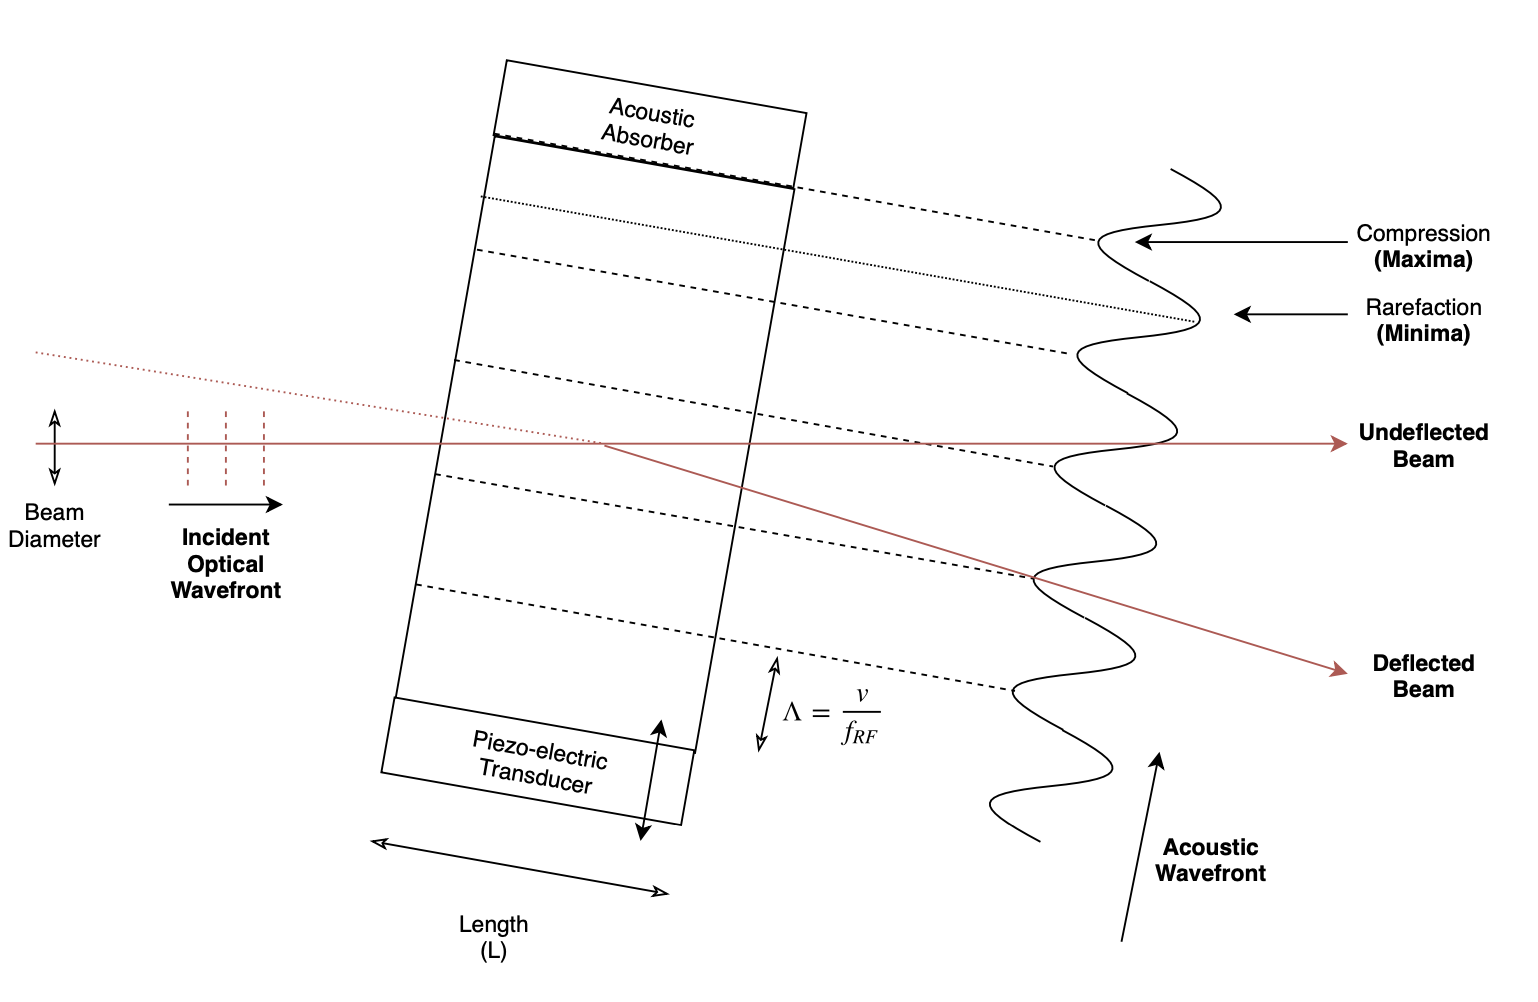
\includegraphics[width = 8cm]{../Figures/aodiagram.png}
    \caption{Diagram showing density fluctuations in medium. The refractive index value varied with the acoustic wave i.e higher 
    refractive indicies occured in areas of compressions and lower indicies in areas of rarefractions of the acoustic wave.}
    \label{fig:aodiagram}
\end{figure}

A simple explanation for these observations points out that the supersonic waves traveling through the crystal periodically varies 
the refractive index of light along the direction perpendicular to the sound wave fronts, causing the light to diffract similar to 
a phase grating, as seen in Figure \ref{fig:aodiagram}, \citep{RamanNath}. Experimentally, the following relationship was obtained,

\begin{equation}
    \sin{\theta} = \pm \frac{n\lambda}{\Lambda}.
    \label{eqn:RamanNath}
\end{equation}

where $\theta$ is the angle between the central beam and the nth order beam, $\lambda$ is the wavelength of light and $\Lambda$ is the 
wavelength of the sound wave.

\begin{figure*}
    \centering
    \subfloat[Bragg diffraction]{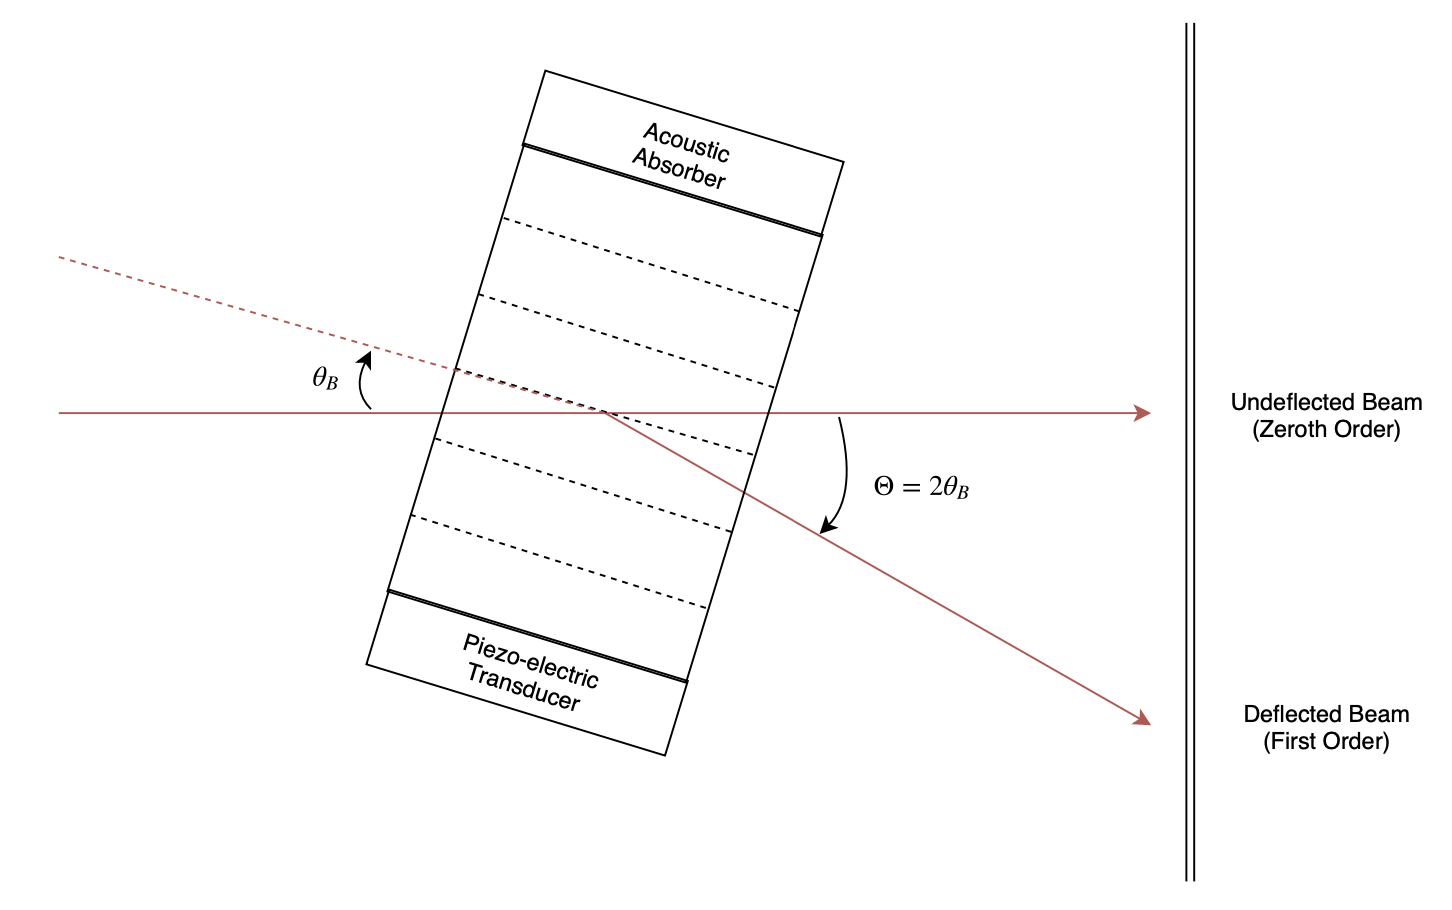
\includegraphics[width=0.5\textwidth]{../Figures/bragg.png}}
    \subfloat[Raman-Nath diffraction]{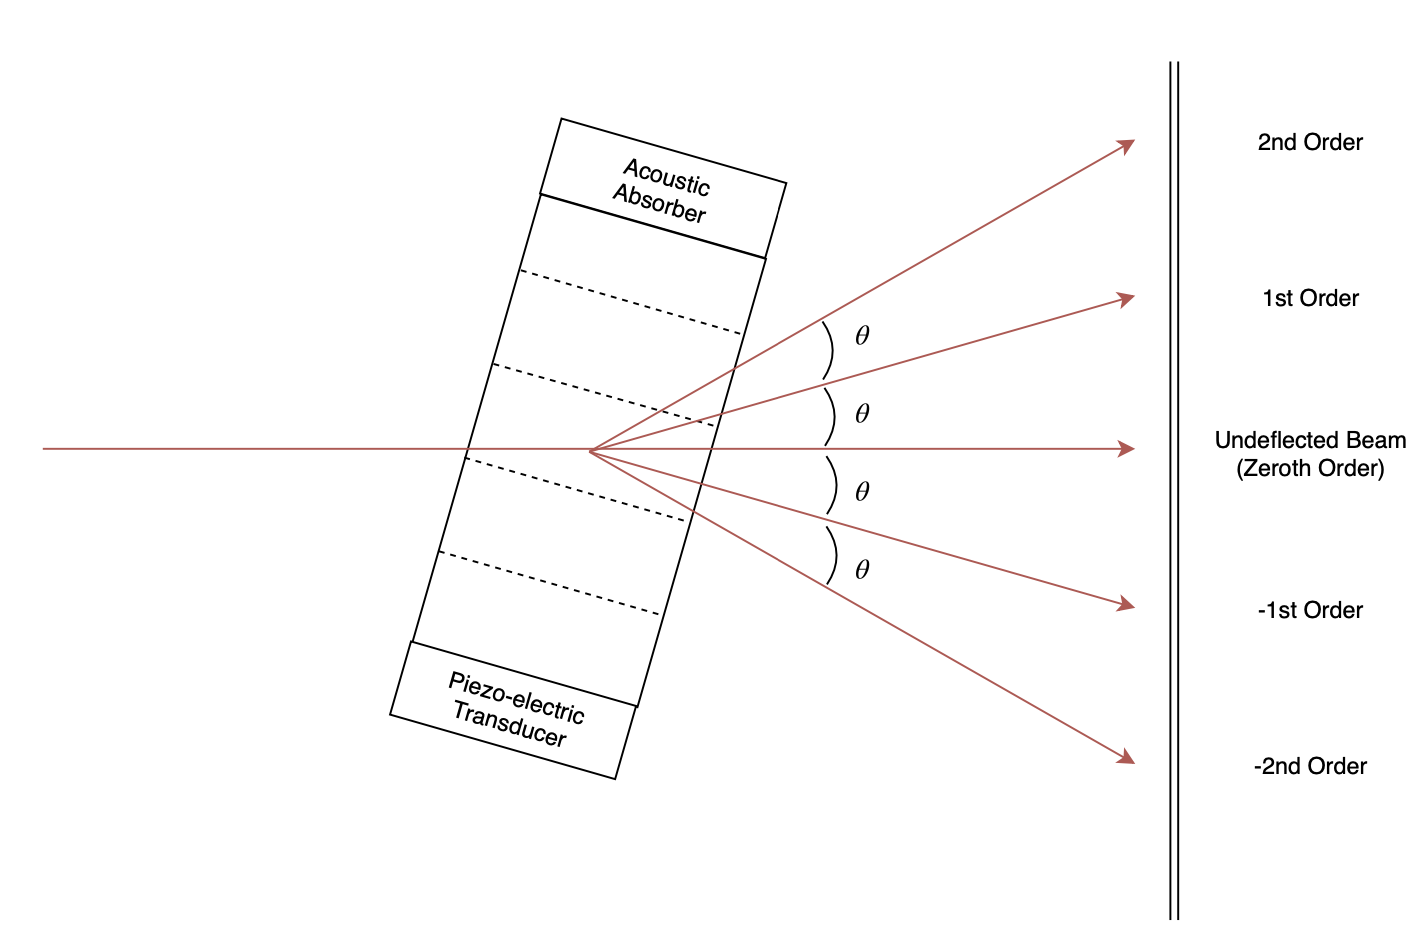
\includegraphics[width=0.5\textwidth]{../Figures/ramannath.png}}
    \caption{Diagram of the two diffraction regimes.}
    \label{fig:diagrams}
\end{figure*}

There are two distinct regimes in acousto-optics, related to the 'thickness' of the diffraction grating induced by the supersonic 
waves. The Raman-Nath regime is observed when the grating is considered to be thin. The resultant diffraction pattern will display 
a number of diffraction maxima symmetrically arranged in a row around the central maxima. This diffraction pattern can be observed 
at any small angle. These two regimes are found in Figure \ref{fig:diagrams}. Conversely, the Bragg regime can only be observed at 
the Bragg angle of light incidence, $\theta_B$, a geometrical approach can be found in the Appendix. The angle can 
be determined by the ratio, \citep{Zakharov},

\begin{equation}
    |\sin{\theta_B}| = \frac{K}{2k} 
\end{equation}

where k and K are the wave numbers of the light and sound waves respectively. The Klein-Cook parameter, $Q$, follows from this, 
traditionally defined as, \citep{Gao},

\begin{align} \label{eqn:kleincook}
    Q &= \frac{K^2 L}{n_0 k \cos\theta} \\
    &\approx \frac{K^2 L}{k} \\
    &= \frac{2\pi \lambda L}{\Lambda^2},
\end{align}

where L denotes the width of the crystal medium. This parameter quantiatively defines these two regimes, Raman-Nath observations 
are said to be in the domain of $Q \ll 1$ whereas the Bragg regime lies in the range of $Q \gg 1$. 

\subsection{\normalfont\textit{Intensity in R-N regime}}
Debye and Sears \citep{DebyeSears} had observed in their initial experiments that when the transducer 
was continuously turned in one direction, starting from a position that gave the highest intensity to 
one of the other orders, the intensity would decrease steadily, goes through zero, increases 
to a value much smaller than the first maximum, goes through zero again and then to another smaller maximum 
and this would repeat.

\section{Aim}

Verify observations of previous experiments and investigate the behaviour of the acousto-optic deflector and modulator to achieve a 
greater understanding of the devices and to understand the difference between Bragg and Raman-Nath Diffraction.

\section{Method}

\subsection{\normalfont\textit{Instruments}}
In this experiment, we used an AO deflector made of dense flint glass and an AO modulator made of lead molybdate. Both devices are capable 
of sending acoustic waves through their respective mediums however their main functions differs. The purpose of a modulator is to modulate 
the intensity or frequency of the diffracted light. This is done by inputting a relative smaller input modulating wave on the order of 
400 Hz, compared to the carrier wave of 110 MHz. This allows us to change the acoustic amplitude whereby we can study the relationship between 
intensity and the acousto-optic effect. The modulator itself will have an acoustic width of approximately 0.8 cm. This is in contrast to a 
deflector whose main purpose is to deflect or steer the diffracted beam, changing its angle. This is achieved with a wider acoustic width of 
11.5 cm allowing for acoustic frequencies on the order of 70-110 MHz to be used as modulating input waves.

The light is said to be modulated when its intensity varies proportional to the peak of the modulating signal. 

\begin{figure}[b]
    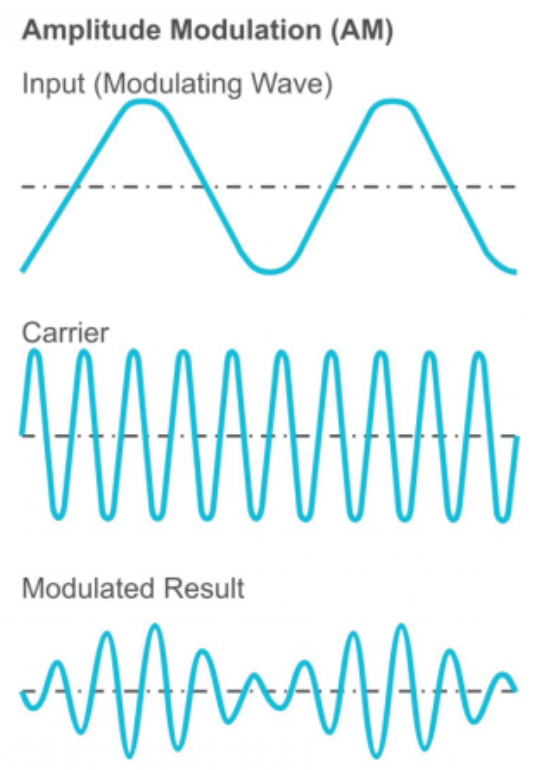
\includegraphics[width=4cm]{../Figures/modulation.png}
    \caption{The modulating wave is created by a superposition of an input modulating wave with a carrier wave.}
    \label{fig:mod}
\end{figure}

The modulating signal is created by combining an input modulating wave from a signal generator with a carrier wave of relatively higher 
frequency as seen in Figure \ref{fig:mod}.

The RF modulator, used for the R-N regime, is specifically designed to work on 28V to produce a 110 MHz carrier wave. Due to limitations of the equipment, these 
parameters cannot be adjusted.

\subsection{\normalfont\textit{Theory}}
We will rewrite Equation \ref{eqn:RamanNath} to obtain a relationship between the Bragg Angle and the frequency of the modulating 
sound waves,

\begin{equation*}
    \sin{\Theta} = \frac{\lambda}{\Lambda}
\end{equation*}

where $\Theta$ is the angle between the zeroth and first diffracted order beams. Substituting in the velocity of sound wave and the Bragg's angle,

\begin{equation*}
    \sin{2\theta_B} = \frac{f_{\text{RF}}\lambda}{v}.
\end{equation*}

We can use the small angle approximation here,

\begin{equation*}
    \sin{2\theta_B} \approx 2\theta_B.
\end{equation*}

We can write,

\begin{align}
    2\theta_B &= \frac{f_{\text{RF}}\lambda}{v} \\
    \theta_B &= \frac{\lambda}{2v}f_{\text{RF}}.
    \label{eqn:velocity}
\end{align}

\subsection{\normalfont\textit{Bragg Angle}}
To determine the Bragg Angle for a 70 MHz signal, the deflector was slowly rotated until a maximum intensity on the screen could be observed.
The distance between the left maxima to the central beam was measured to be $1.80 \pm 0.05$ cm. Similarly the right maxima 
to the central maxima was measured to be $1.85 \pm 0.05$ cm. The average distance, $d$, is then $1.83 \pm 0.07$ cm. The distance 
of the deflector, $L$, was measured to be $159.0 \pm 0.1$ cm. The Bragg Angle is then,

\begin{align*}
    \theta_B &= \tan^{-1}\left(\frac{d}{L}\right) \\
    &= 0.0115 \pm 0.0004\text{ rad} \\
    &= 11.5 \pm 0.4 \text{ mrad}.
\end{align*}

This represents a 0.8\% error from the specification provided by the deflector manual, citing the beam separation for a 70 MHz signal to be $11.4$ mrad. 
Therefore our value agrees with the predetermined specifications.

\subsection{\normalfont\textit{Acoustic Velocity}}

To find the acoustic wave for the Acousto-Optic modulator at 110 MHz. We can use Equation \ref{eqn:RamanNath}, but now solving for $v$. The distance from the 
modulator to the screen was measured to be $162 \pm 0.1$ cm. The distance from the central beam to the left 1st order maxima was $3 \pm 0.05$ cm. Similarly, 
the distance to the right maxima was $3.1 \pm 0.05$ cm. This gave an average angle of $0.0188 \pm 0.000618$ rad. Substituting into the Equation \ref{eqn:RamanNath},
where $f_{\text{RF}} = 110 \text{ MHz}$,

\begin{equation*}
    \sin{\theta} = \frac{\lambda}{\Lambda}.
\end{equation*}

Applying a small angle approximation and rewriting $\Lambda$ as $\frac{v}{f_{\text{RF}}}$,

\begin{align*}
    \theta &= \frac{f_{\text{RF}}\lambda}{v} \\
    v &= \frac{f_{\text{RF}}\lambda}{\theta} \\
    &= \frac{110 \times 10^6 \times 633 \times 10^{-9}}{0.0188} \\
    &= 3754 \pm 124 \text{ ms}^{-1}.
\end{align*}

This represents a 3.4\% deviation from the specified acoustic velocity obtained from the modulator manual. However this deviation 
is accounted for by the uncertainty of the measurement.

We can then check the Klein-Cook parameter found in Equation \ref{eqn:kleincook}, rewriting the wavelength of the acoustic wave to 
involve its velocity,

\begin{equation*}
    Q = \frac{2\pi \lambda L f_{\text{RF}}^2}{v^2},
\end{equation*}

substituing in our values,

\begin{align*}
    Q &= \frac{2\pi (633\times10^{-9})(0.8\times10^{-2})(400)}{3754^2} \\
    &= 3.42 \times 10^{-10} \\
    &\ll 1.
\end{align*}

We can definitively determine that we are in the Raman-Nath regime.

\subsection{\normalfont\textit{Intensity in R-N Regime}}
Taking an analytical treatment of the problem, Raman and Nath \citep{RamanNath} found a relationship for the relataive intensity of the diffracted light 
that followed the observations of Debye and Sears,

\begin{equation} \label{eqn:ramannath}
    I_1 \propto J_1^2\left(\Delta\phi \sec{\theta} \frac{sin(\pi W \tan{\theta}/\Lambda)}{\pi W \tan{\theta}/\Lambda}\right).
\end{equation}

The existence of a Bessel function suggests a radial component to the acoustic diffraction. Although the aperture is a lot more complicated, we can abstract 
away the sophistication and think of the problem as an example of Fraunhofer diffraction. We can check the Fraunhofer condition to ensure that Fraunhofer 
diffraction is valid,

\begin{equation} \label{eqn:fraunhofer}
    \frac{(x^2+y^2)}{2\lambda R_0} \ll 1.
\end{equation}

From the specifications, we find that the active aperture of the lead molybdate crystal to be 1 mm, checking the far field condition

\begin{align*}
    \frac{{x^2+y^2}}{2\lambda R_0} &= \frac{(1\times10^{-3})^2}{2(633\times10^{-9})(162\times10^{-2})} \\
    &= 0.48
\end{align*}

we cannot say definitively that the Fraunhofer condition is satisfied as the statement $0.48 \ll 1$ is not true to a strong enough extent.

The resulting Bessel function could then be thought of as a consequence of a Hankel transform required to compute the integral in the Fraunhofer diffraction equation. However 
experimentally, the Fraunhofer condition is not completely satisfied and so the resulting intensity diffracted field may not be observed.

\section{Results \& Analysis}
\subsection{\normalfont\textit{Bragg Regime}}

\begin{figure}
    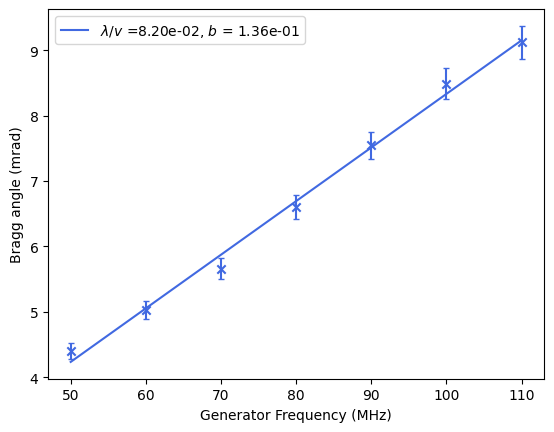
\includegraphics[width = 8cm]{../Figures/velocity.png}
    \caption{Linear function of the measured Bragg angle as the frequency in the deflector was increased 
    slowly from 50MHz to 110MHz.}
    \label{fig:velocity}
\end{figure}

The velocity of the acoustic wave in the deflector was calcuated using Equation \ref{eqn:velocity}. Referring to Figure \ref{fig:velocity}, and applying the appropriate scaling factors,

\begin{align*}
    \frac{\lambda}{2v} &= 8.20 \times 10^{-2} \times \frac{10^{-3}}{10^{6}} \\
    v_{\text{sound}} &= \frac{633 \times 10^{-9}}{2\times8.20 \times 10^{-11}} \\
    &= 3859.8 \pm 134\text{ ms}^{-1}
\end{align*}

We can now check the Klein-Cook parameter, $Q$, as defined in Equation \ref{eqn:kleincook}, rewriting using the velocity of the acoustic wave,

\begin{equation*}
    Q = \frac{2\pi\lambda Lf_{\text{RF}}}{v}.
\end{equation*}

Substituting in our values,

\begin{align*}
    Q &= \frac{2\pi (633\times10^{-9})(11.5\times10^{-2})(110\times10^6)^2}{3859.8^2} \\
    &= 371 \\
    &\gg 1.
\end{align*}

Therefore, we are definitively in the Bragg Regime.

\begin{figure}
    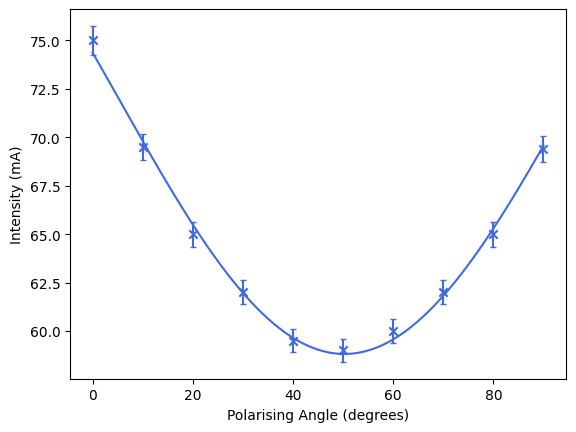
\includegraphics[width = 8cm]{../Figures/polarisation.png}
    \caption{Parabolic function displaying the relationship between the diffracted intensity and the 
    polarisation of the incident light.}
    \label{fig:polarisation}
\end{figure}

We also found that the polarisation of incident light on the deflector influenced the intensity of the diffracted light. The intensity of the diffracted beams followed 
Malus' Law, as seen in Figure \ref{fig:polarisation},

\begin{equation} \label{eqn:malus}
    I = I_0\cos^2{\theta},
\end{equation}

indicating that the only factor affecting the peak intensity of the diffracted beams was the intensity and the polarisation of the incident beam. The deflector and acoustic waves 
were purely changing the phase of the light, not its intensity behaviour in any significant way other than a simple offset.

\subsection{\normalfont\textit{Raman-Nath Regime}}

\begin{figure*}
    \centering
    \subfloat[Under Modulation]{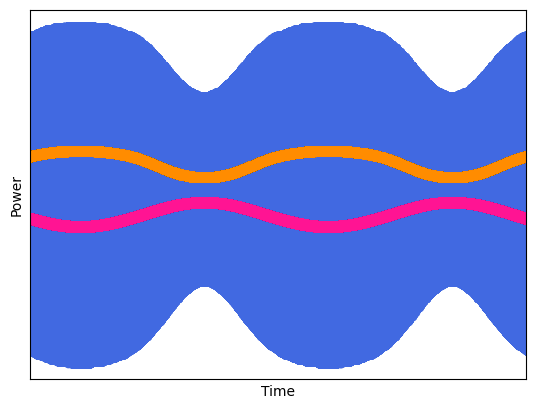
\includegraphics[width=0.45\textwidth]{../Figures/lowmodplot.png} \label{fig:sub1}}
    \subfloat[Full Modulation]{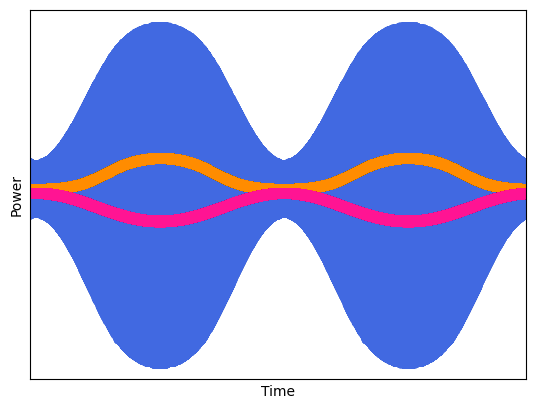
\includegraphics[width=0.45\textwidth]{../Figures/fullmodplot.png} \label{fig:sub2}} \\
    \subfloat[Over Modulation]{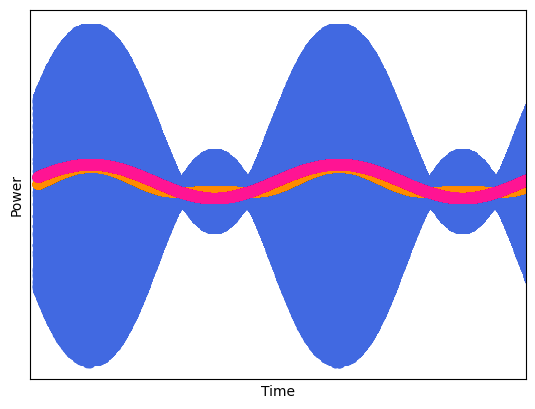
\includegraphics[width=0.45\textwidth]{../Figures/overmodplot.png} \label{fig:sub3}}
    \subfloat[Modulating with rap song 'Tweaker']{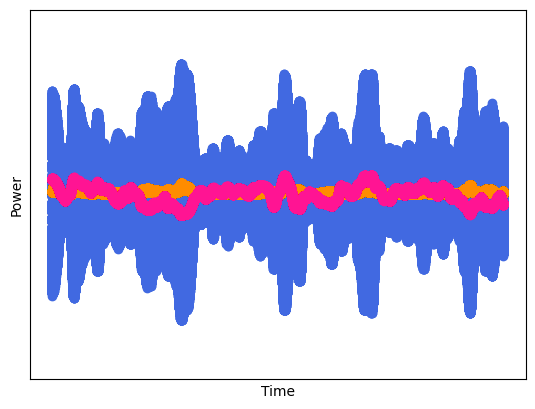
\includegraphics[width=0.45\textwidth]{../Figures/geloplot.png} \label{fig:sub4}}
    \caption{Four figures that display the combination of the modulating input wave (pink), the modulating result (blue)
    and the intensity of the diffracted beam (orange). Note that the input wave is out of phase with the other two in (a) and (b),
    this simply results in a vertical offset in the resulting wave as the carrier wave has much higher frequency than the input wave 
    so when combined, the input wave can be approximately thought of as constant. The overmodulation in (c) reduces the total dominance 
    in amplitude of the carrier wave so the resulting intensity of the diffracted beam is now more in phase with the input wave. In (d), 
    the input wave is not periodic so the resulting intensity is also not periodic but is also out of sync with the input wave due to the 
    carrier wave.}
    \label{fig:main}
\end{figure*}

When an acoustic wave is put through the crystal transducer, the density of the solid changes. A laser beam passing through this pressure changing medium would see its ray of light 
interact with periodic changes in the refractive index, causing the light to effectively diffract. We put waves varying in their modulation through the crystal and qualitatively 
observed the effects of different modulations on the intensity of the diffracted beam. The carrier wave of 110 MHz was kept the same however the offset of the input modulating wave 
was changed to simulate the effect of different wave modulations. We found that under and over modulations drastically affected the phase of the resulting intensity. In the case of 
under modulation, the periodic changes in the intensity of the diffracted beam was exactly out of phase with the input modulating wave as seen in the top left panel in Figure \ref{fig:main}.
This would also be seen in the case of proper full modulation, however when the input modulating wave was under modulated, there was a clear vertical offset in the resulting periodic intensity 
in comparison to the input modulating signal, which should be kept constant throughout all the panels. The amplitude being kept high due to under modulation would cause the significant 
vertical offset. The vertical offset is no longer seen in the top right panel as the amplitude of the modulating wave is significantly small enough in the region where the input modulating 
wave and the resulting periodic intensity's zeroes coincide. The shape of the periodic intensity of the diffracted beam changes in the case of the over modulated wave. This is beecause 
the modulating wave picks up a new 'wavepacket' that is an artifact of increasing the offset to a high enough threshold where the phase difference between the carrier wave and the input 
modulating wave produces stranger periodic patterns. This is more clearly seen in Figure \ref{fig:compare}. This artifact effect is more accentuated in inputing a less periodic signal such as from a song or random sound. We played the popular rap 
song 'Tweaker' by GELO, through an aux input into the crystal transducer and produced the graph in the bottom right panel. Despite the random nature of the input modulating wave, the resulting 
modulated wave produces periodic patterns that should not arise given the input signal. 

\begin{figure*}
    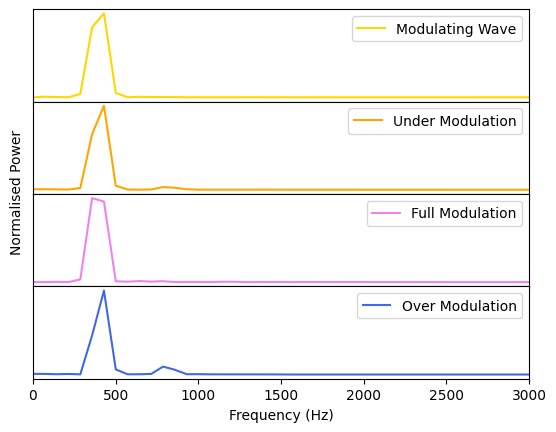
\includegraphics[width = 12cm]{../Figures/comparefft.png}
    \caption{Plot of the under (orange), full (pink) and over (blue) modulated result, compared with each other 
    and the input modulating wave (yellow). The peak frequency of the signal wave , under, full and over modulating 
    waves are 428.87 Hz, 430.49 Hz, 429.08 Hz and 428.65 Hz respectively. There is a secondary peak in the over modulated 
    wave at 642.98 Hz. The full width at half maximum (FWHM) for all peaks are approximately 214 Hz.}
    \label{fig:compare}
\end{figure*}

We can more quantiatively analyse the acoustic effects by plotting the previous figures in Fourier space. We find that experimentally, we wanted to input a 400 Hz modulating wave but due to 
uncertainties in the instrumentation, we find that the actual frequency of the input was closer to 430 Hz. We can also define an uncertain for this experiment by using the FWHM value which 
was the same for all readings using the following Gaussian assumption,

\begin{equation}
    \sigma = \frac{\text{FWHM}}{2\sqrt{2\ln{2}}}.
\end{equation}

This gives us a frequency uncertainty for all readings to be approximately $\pm$ 91 Hz. This explains the strong deviation away from the expected input modulating wave signal to be 400 Hz.
Nevertheless, we find that despite the varying modulations, the peak frequency of the periodic intensity corresponds to the input modulating wave frequency to a high accuracy. The aforementioned 
artifact is found at 642.98 Hz in the over modulated result. The position of the artifact is based on the phase difference between the input modulating wave and the carrier wave.

\subsubsection{Different waveforms}

\begin{figure} [!htbp]
    \subfloat[Plot of the power of the diffracted beam versus time for a square input modulating wave.]{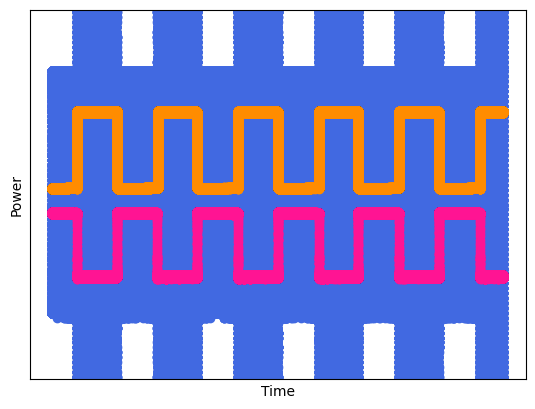
\includegraphics[width=8cm]{../Figures/squareplot.png}} \\
    \subfloat[Power spectrum of the above plot. Notice the artifact at ~1200 Hz]{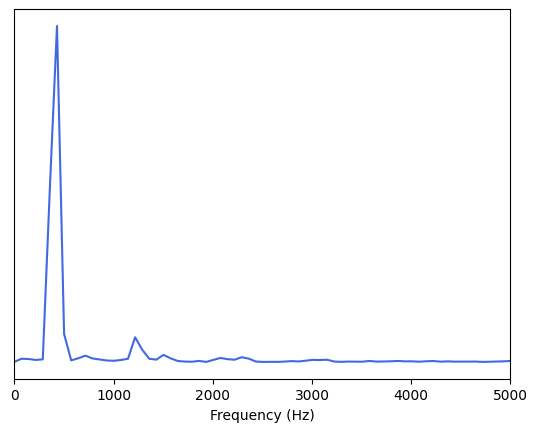
\includegraphics[width=8cm]{../Figures/squarefourier.png}}
    \caption{Pair of plots for square modulated wave}
    \label{fig:square}
\end{figure}

\begin{figure} [!htbp]
    \subfloat[Plot of the power of the diffracted beam versus time for a triangle input modulating wave.]{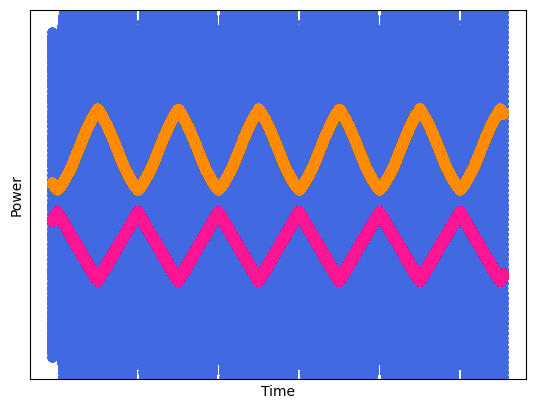
\includegraphics[width=8cm]{../Figures/spikyplot.png}} \\
    \subfloat[Power spectrum of the above plot]{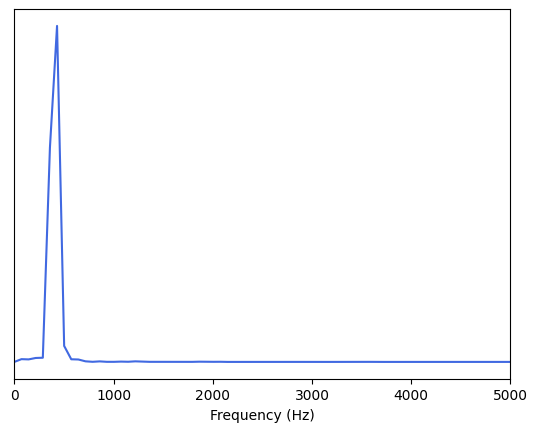
\includegraphics[width=8cm]{../Figures/spikyfourier.png}}
    \caption{Pair of plots for triangle modulated wave}
    \label{fig:triangle}
\end{figure}

\begin{figure} [!htbp]
    \subfloat[Plot of the power of the diffracted beam versus time for a 800 Hz sine wave.]{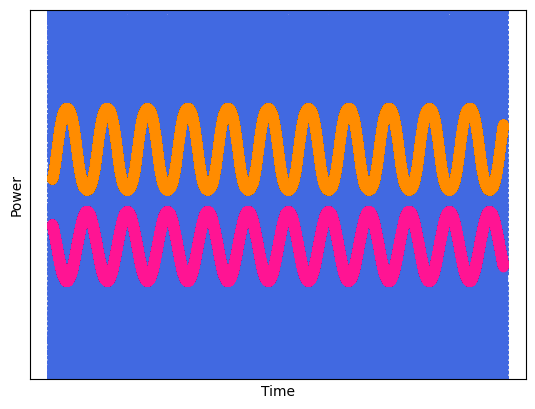
\includegraphics[width=8cm]{../Figures/sine800plot.png}} \\
    \subfloat[Power spectrum of the above plot. As expected, the peak frequency is ~800 Hz]{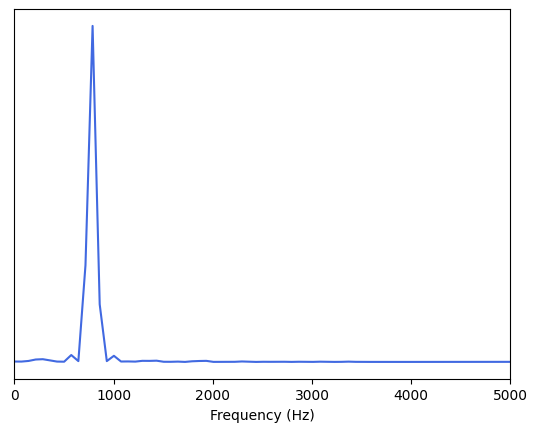
\includegraphics[width=8cm]{../Figures/sine800hzfourier.png}}
    \caption{Pair of plots for twice the frequency sine wave for modulated wave}
    \label{fig:800sine}
\end{figure}

We replaced the 400 Hz sine wave input modulating wave with different waveforms and plotted their power over time in the Figures \ref{fig:square}, 
\ref{fig:triangle} and \ref{fig:800sine}. In the case of the square input wave, we find that the carrier wave is modulated appropriately as the offset 
from the input wave is large enough to modulate the carrier wave. Plotting this in Fourier space reveals a secondary peak at ~1200 Hz. This would likely 
be due to overmodulation due to the shape of the waveform. For the triangle waveform, we find that the shape of the input modulating wave is conserved. 
However, due to the shape of the waveform, we find that the carrier wave is not modulated. This is likely due to the weak modulating strength of the shape, 
relative to the frequency used. It can be postulated that if the frequency was turned down, the carrier wave would be more appropriately modulated. In Fourier 
space, we find no strange occurences that deviate from expected results. Finally, doubling the frequency to 800 Hz, drastically under modulated the carrier wave.
To counter, we would need to increase the offset appropriately. As expected, the intensity peak in Fourier space appears at 800 Hz.

\subsubsection{SMVR}

The speaker was attached to the photodiode measuring the intensity of the diffracted beam. The signal to mean value ratio (SMVR) was then calculated for the diffracted beam and the main beam by 
taking the ratio of the peak to peak voltage of the AC coupling to the mean voltage of the DC coupling of the signal. The main beam measured a SMVR value of 0.046 whilst the diffracted beam 
measured a value of 2.2. The speaker when connected to the diffracted beam, played distorted sounds in addition to the original 'Tweaker' song that was inputed into the modulating wave. When we 
connected the speaker to the main beam, we found no distortions and the original input signal of the song was recovered fully. We tentatively can say that the SMVR of the signal is indicative of 
the strength of the signal, i.e a lower SMVR ratio means that the measured wave has a stronger signal. As a fun qualitative experiment, we changed the input modulating wave back to the signal 
generator but still with the speaker connected. This lead to a sound with a pitch dependent on the frequency of the input wave, as expected. We increased the frequency of the input wave to the 
point where we could both no longer hear the sound, we found this frequency to be 18800 Hz which corresponds to the known upper value for the human hearing range. 

\subsubsection{Intensity}

In this section, we want to verify the observations found initially by Debye and Sears \citep{DebyeSears} and later quantiatively described by Raman and Nath \citep{RamanNath}. The intensity of 
the acoustically diffracted optical beam can be described by Fraunhofer diffraction by modelling the transducer as a diffraction grating. However, due to equipment limitations, the size of the 
aperture is relatively large whilst the distance between the observation and aperture plane is too small as to not satisfy the Fraunhofer condition as seen in Equation \ref{eqn:fraunhofer}. Hence, 
we will expect to not see a perfect diffracted intensity pattern but will still proceed with the experiment to see how much of the effects described by Debye and Sears are retained despite unideal 
conditions. Furthermore, the intensity pattern of the diffracted field is best probed by changing the diffracting power of the acoustic wave i.e by increasing the frequency of the carrier wave, 
\citep{Zakharov}, \citep{Gao} and \citep{Kwiek}. These papers effectively reproduced the diffracted field intensity pattern by changing the phase shift of the optical wave, denoted by the $\Delta \phi$
in the Raman Nath equation, Equation \ref{eqn:ramannath}. This parameter is known as the Raman-Nath parameter and can be expanded into 

\begin{equation}
    \Delta \phi = k \frac{\partial n}{\partial p}p L
\end{equation}

where $k$ is the wave number of the light wave, $\frac{\partial n}{\partial p}$ is the differential of the refractive index, $n$, with respect to the sound pressure amplitude, $p$ and $L$ is the sound 
field depth. By increasing the frequency of the acoustic wave, the $\frac{\partial n}{\partial p}$ term will increase, increasing the Raman-Nath parameter as a whole. The aforementioned constraint of the 
carrier wave being only limited to 110MHz disallows us to perform the same experiment. Furthermore, we were unable to increase $R_0$ far enough to achieve far field diffraction so we will simply just rotate 
the angle of incidence of the optical beam onto the crystal and try to observe any changes in intensity.

\begin{figure}[!htbp]
    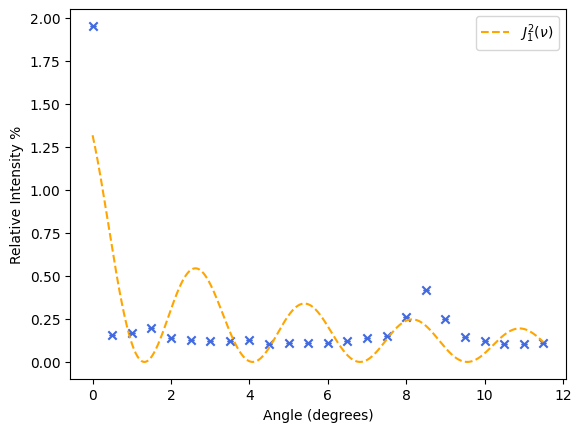
\includegraphics[width = 8cm]{../Figures/intensity.png}
    \caption{Plot of relative intensity of the diffracted beam and the undiffracted main beam versus the angle of incidence of the laser beam onto the 
    surface of the crystal. Starting from the peak intensity and going towards one direction, we expect a periodic increase and 
    decrease in intensity going to zero and then peaking again at some smaller maximum, as seen in the dotted orange line. We find that experimentally, 
    this was not the case. Rather, there was a peak at the normal incidence and then at the 8-8.5 degree point. Error bars are plotted but are insignificant 
    as the uncertainty is on the order of 0.005\%. The statistical uncertainty was calculated using the standard deviation of the mean value of the voltage 
    as read by the photodiode over 100 counts.}
    \label{fig:intensity}
\end{figure}

Immediately from Figure \ref{fig:intensity} we are able to see an unexpected result. There is a clear maximum peak of intensity at the 8 to 8.5 degree mark. To check for any random misalignments or fluctuations,
we tried to reproduce this reading by varying the frequency of the input modulating wave as well as the shape of the wave. This maximum occurred for different frequencies and were the same across for the sine, square 
and triangle waveforms. Plotting a theoretical intensity model, the first order Bessel function squared, $J_1^2(\nu)$, we are able to tentatively state that the maximum somewhat coincides with the third order maximum 
of the diffracted intensity field. The possible reason for this occuring could be due to the low resolution of the intensity pattern due to the far field diffraction condition not being met. Information is lost if the 
condition is not met so the pattern we experimentally observed here could just be the intensity pattern with a lot of missing features. The rest of the intensity pattern looks relatively flat however we can zoom into 
these areas by ignoring the maximum intensity at angle 0, shown in Figure \ref{fig:intensity2}.

\begin{figure}[!htbp]
    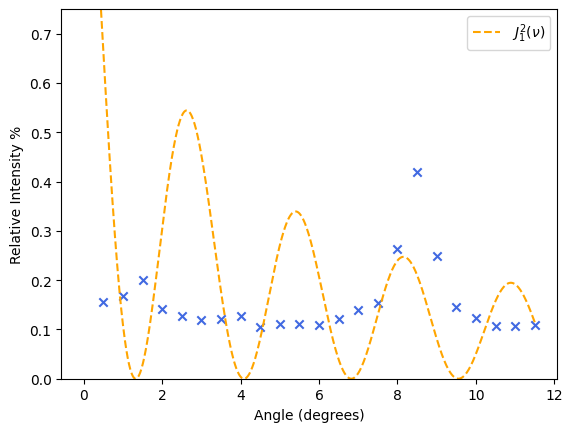
\includegraphics[width = 8cm]{../Figures/intensity2.png}
    \caption{Zooming into the lower half of the previous graph by restricting the 
    vertical axis limit to 0.8\%. We can see that there are small fluctuations in 
    intensity as the angle of incidence increases, indicating some periodic relationship 
    between the intensity and the angle as observed by Debye and Sears and predicted by 
    Raman and Nath.}
    \label{fig:intensity2}
\end{figure}

We can start to see a more expected varying pattern when we look closer at the flatter parts of the experimental data. We find a periodic pattern of maxima and minima agreeing with the observations done by Debye and Sears.
We suspect that the lack of signal from the variations is due to the far field diffraction condition not being met and so the pattern is lacking in certain features, such as these one. The information in the field is still there 
but not strongly accentuated so it results in a pattern with some expected variation but low overall intensity in these areas.

\begin{figure} [!htbp]
    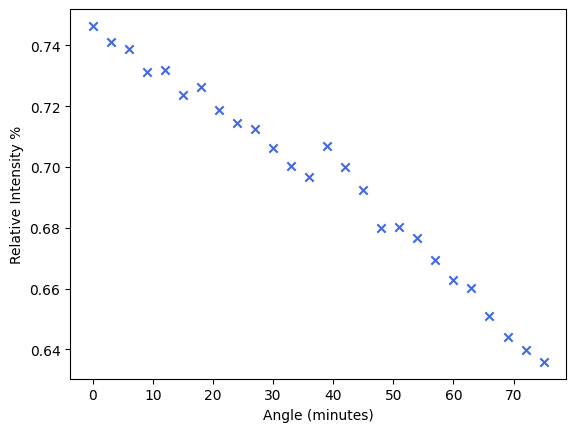
\includegraphics[width = 8cm]{../Figures/intensity3.png}
    \caption{Plot of the small range of 1.25 degrees beginning from the normal incidence. We find that the intensity decreases monotonically suggesting 
    little periodic variation at this small resolution.}
    \label{fig:intensity3}
\end{figure}

Due to small increment steps, we could not see a lot of the intensity changes in the pattern within the first half degree from the maximum intensity point in the previous two figures. We probed this small range using a micrometer
in Figure \ref{fig:intensity3} and found a monotonically decreasing relationship between the intensity and the angle in minutes, which is expected as the intensity drastically drops seen in Figure \ref{fig:intensity}.

\section{Discussion \& Further research}

Our study into acousto optics aptly varied the observations that came before us and provided deeper insights into the acousto-optic effect. We set out to understand the difference between modulators and deflectors. This was achieved 
by computing the Klein-Cook parameter for each instrument and finding that they operated into two difference acousto-optic regimes. The acoustic width or optical depth of the medium was the defining factor for each instrument and it 
enabled two different orders of magnitude of input modulating waves (400 Hz vs 70-110 MHz) to be inputted into the crytals. We successfully and accurately determined that the polarisation had no unexpected effects on the diffracted 
intensity as it followed Malus' Law as if it were just any other polarised light. The Bragg angle for the deflector for a 70 MHz signal was determined to be $11.5 \pm 0.4$ mrad, which agreed with specification values and thus verified 
the theory behind the Bragg regime. 

The Raman-Nath regime proved to be a lot more interesting as the relationship between the power or intensity of the diffracted beam with the angle of incidence or phase shift from the diffraction 
proved to be harder to verify experimentally. We want to revisit this regime with better equipment. The constraint of only applying a 28V power supply to the modulator limited our ability to vary the 
diffracting power. Nevertheless, we were able to explore the impact of phase shifts in the input modulating wave on the resulting modulating wave, finding an interesting artifact in frequency space 
for over-modulation.

The intensity of the diffracted field seemed to be a lot more complicated than a simple Fraunhofer diffraction problem with a diffraction grating as it had some radial symmetry. This isotropic characteristic 
is not found in all crystals and some papers redefine the Klein-Cook parameter and the Raman-Nath intensity relationship for acoustically anisotropic media, \citep{Zakharov}. This would prove to be a great area for further research. 
Other papers, \citep{Kwiek}, explore the relationship between the Klein-Cook parameter, the Raman-Nath parameter and the intensity of the diffracted beam and found strange multi-dimensional relationships. Finally, more practical papers, 
\citep{Kotov}, look to optimise the acousto-optic effect to better improve its applications in general laser beam control, optical information processing and spectroscopy.

\section{Conclusions}

We investigated the difference between acousto-optic modulators and deflectors through analysing the Klein-Cook parameter, finding that the acoustic width of the crystal in the instrument determined the regime in which the acousto-optic 
effect was operating in. Exploring the various relationships between light and the angle enabled us to develop a more well rounded understanding of the Bragg and Raman-Nath regimes.

\section{Appendix}
\subsection{\normalfont\textit{Geometric approach to Bragg Angle}}
\begin{figure}
    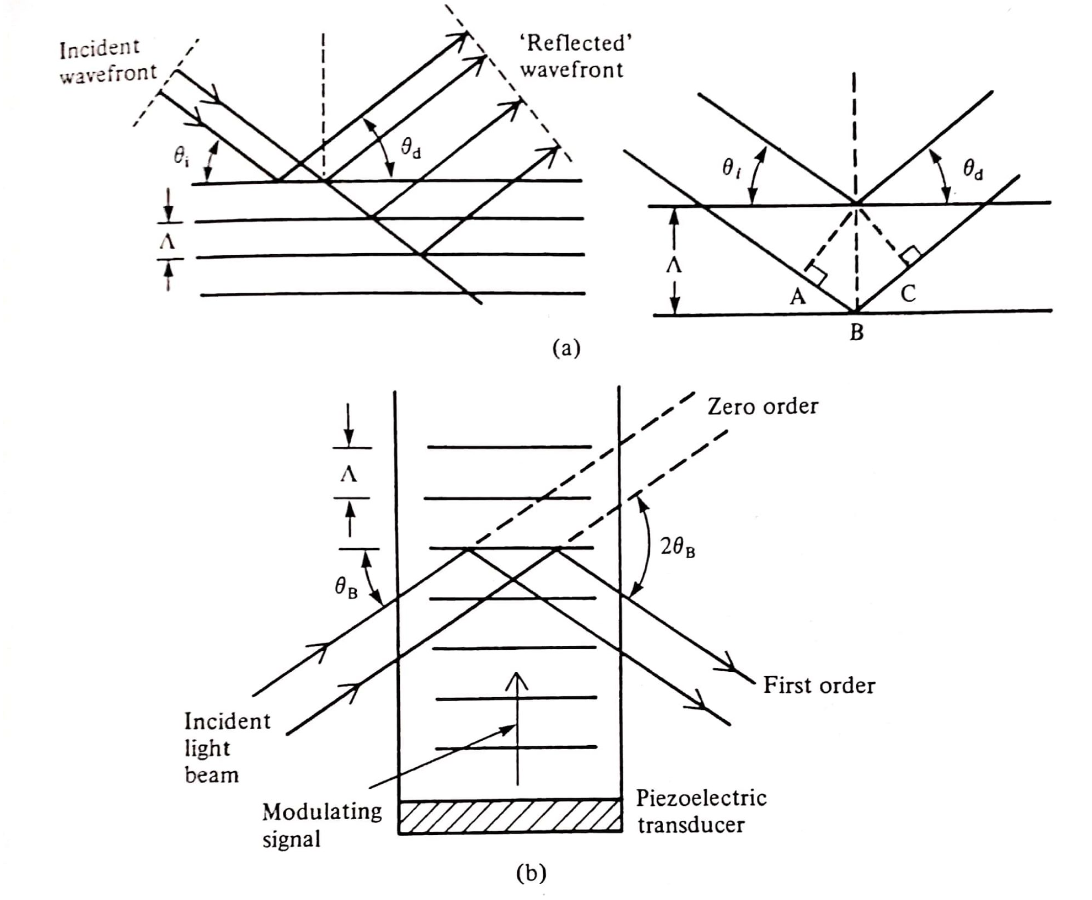
\includegraphics[width=8cm]{../Figures/braggangle.png}
    \caption{Geometric diagram showing ray tracing of light. Bragg deflection occurs when the angle of incident is equal to the angle of the deflected beam}
    \label{fig:geometricproof}
\end{figure}

From a geometric perspective, the Bragg angle occurs when the deflected angle is the same as the angle of incidence on the plane of the sound wave as seen in Figure 
\ref{fig:geometricproof}. The total path difference at the points of constructive interference are then 

\begin{equation}
    \sin{\theta_i} + \sin{\theta_d} = \frac{m\lambda}{\Lambda}.
\end{equation}

As the medium is continuous and not made up of discrete planes, the only point that be viewed is when $m = 1$, so,

\begin{align*}
    2\sin{\theta_B} &= \frac{\lambda}{\Lambda} \\
    \sin{\theta_B} &= \frac{\lambda}{2\Lambda}
\end{align*}

\section{Lab Book}
\begin{figure*}[!htbp]
    \centering
    \subfloat[]{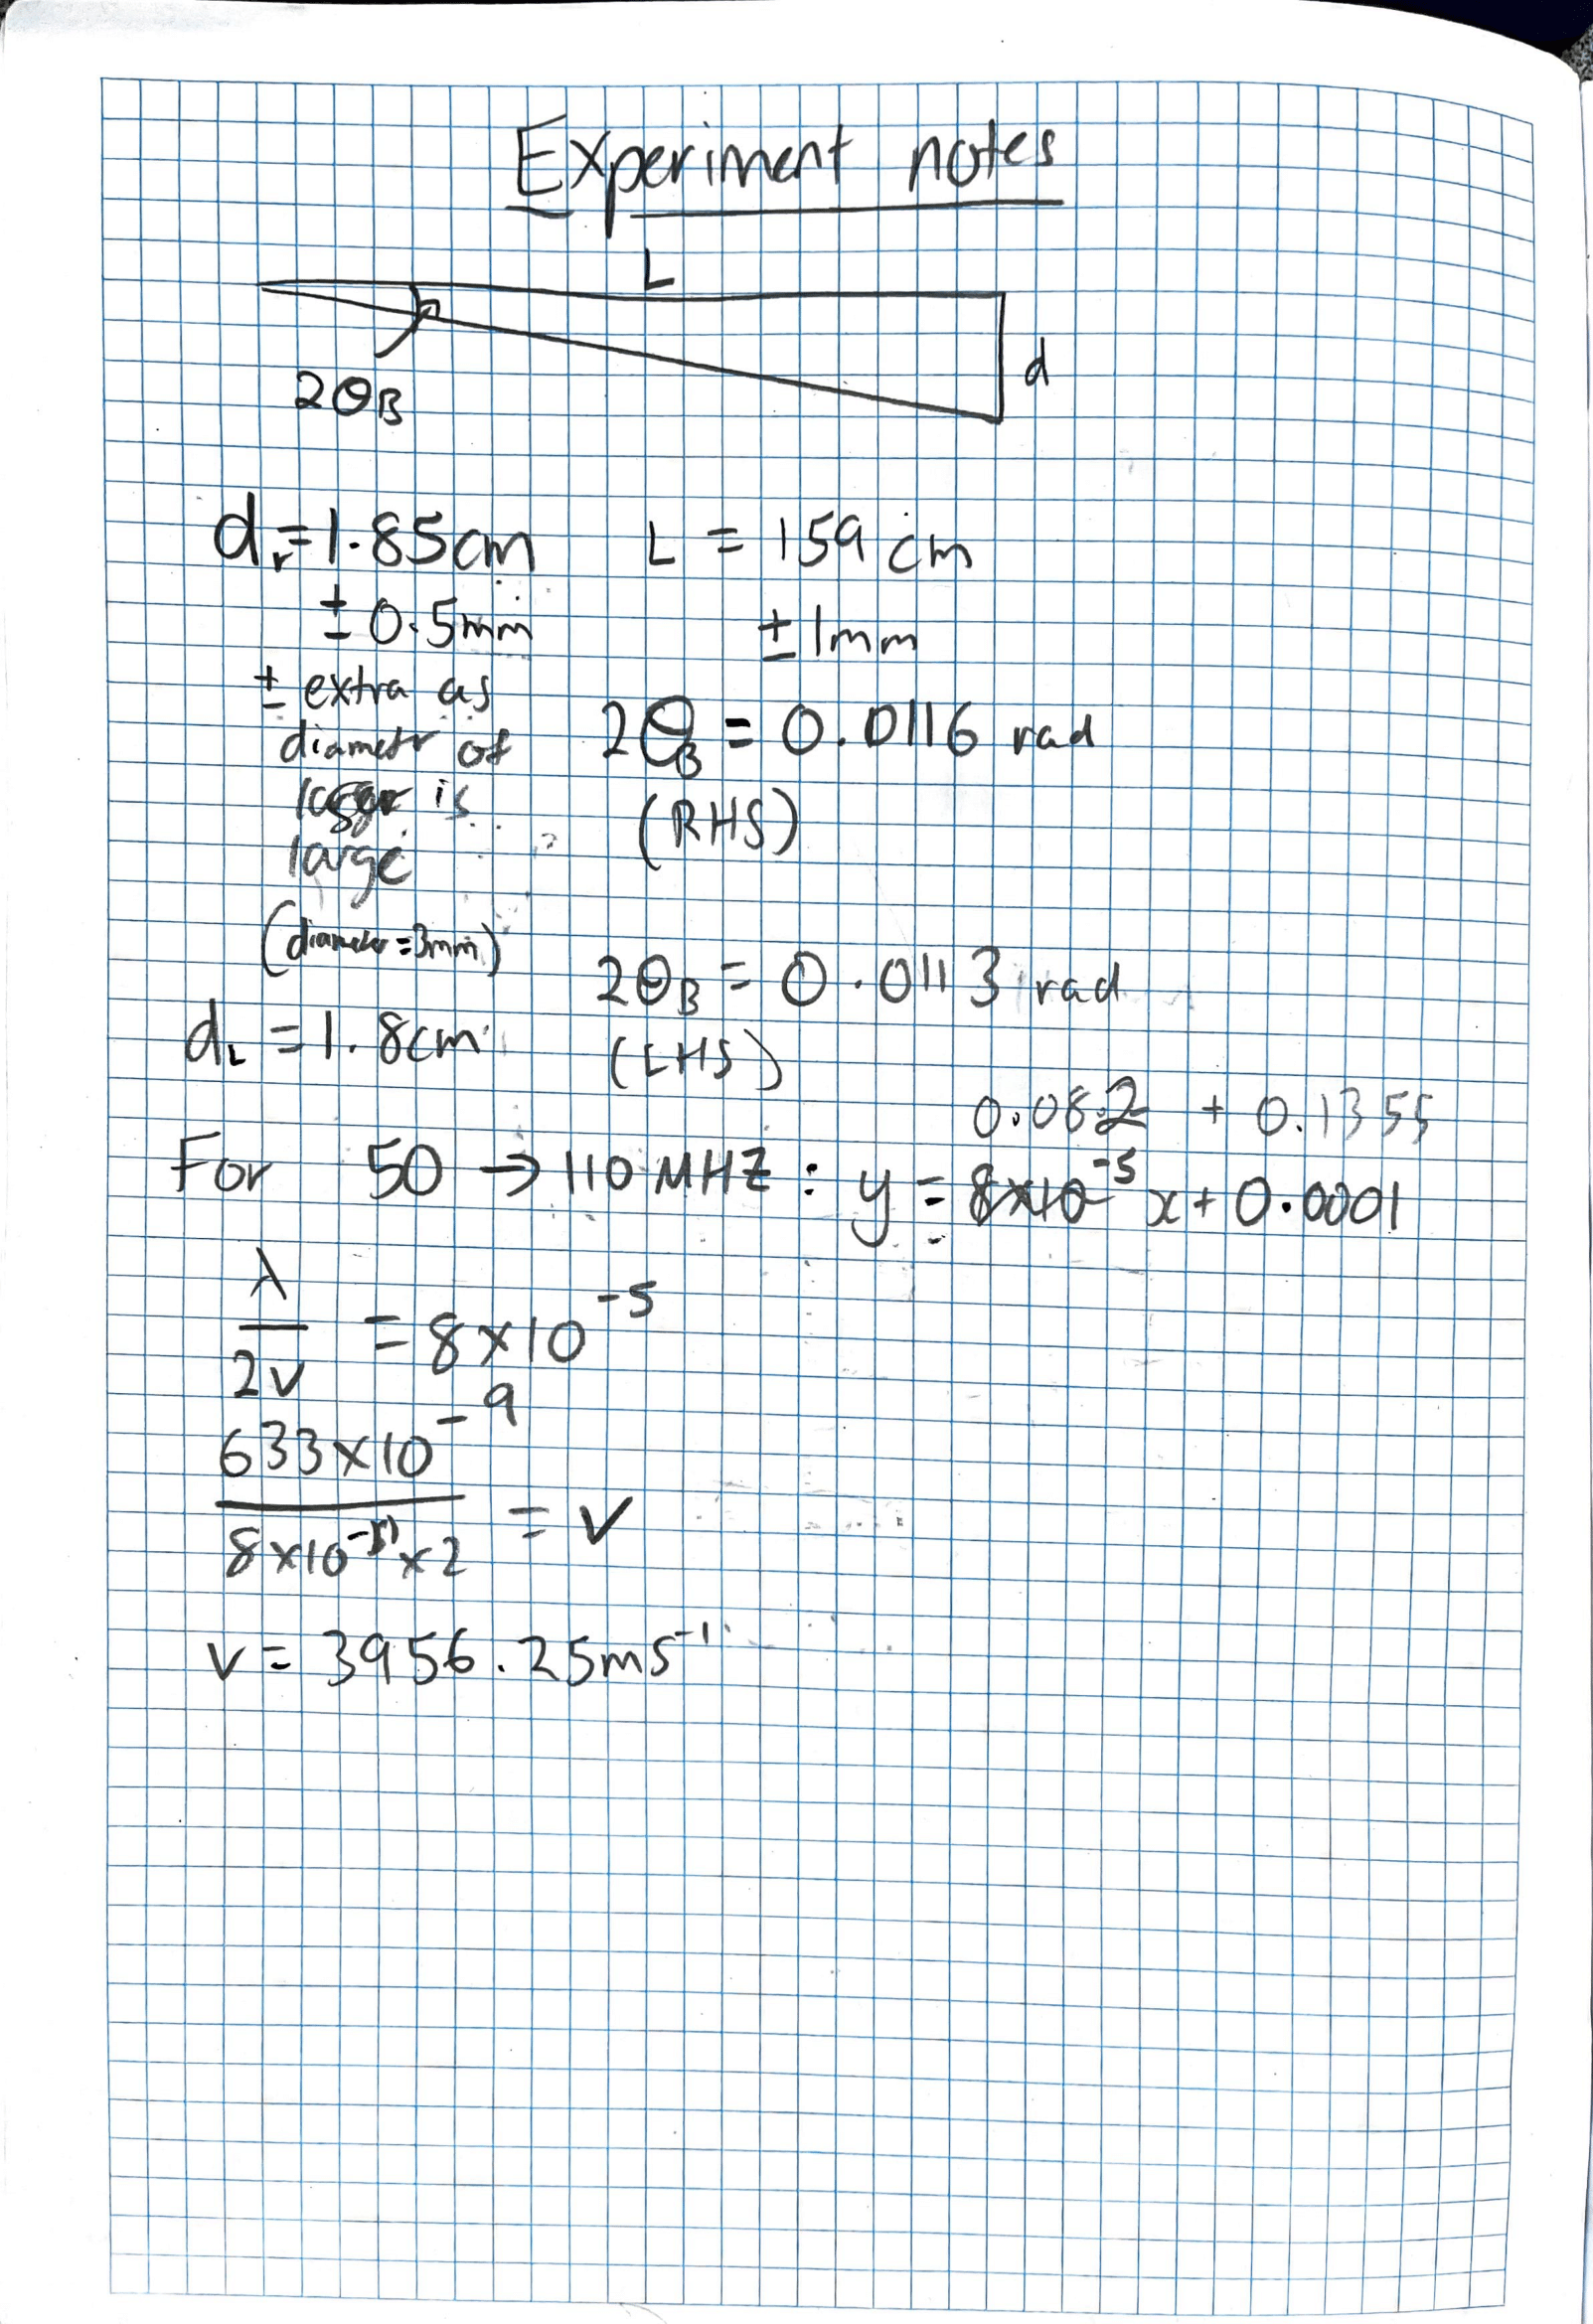
\includegraphics[width=0.3\textwidth]{../Figures/labbook1.png}}
    \subfloat[]{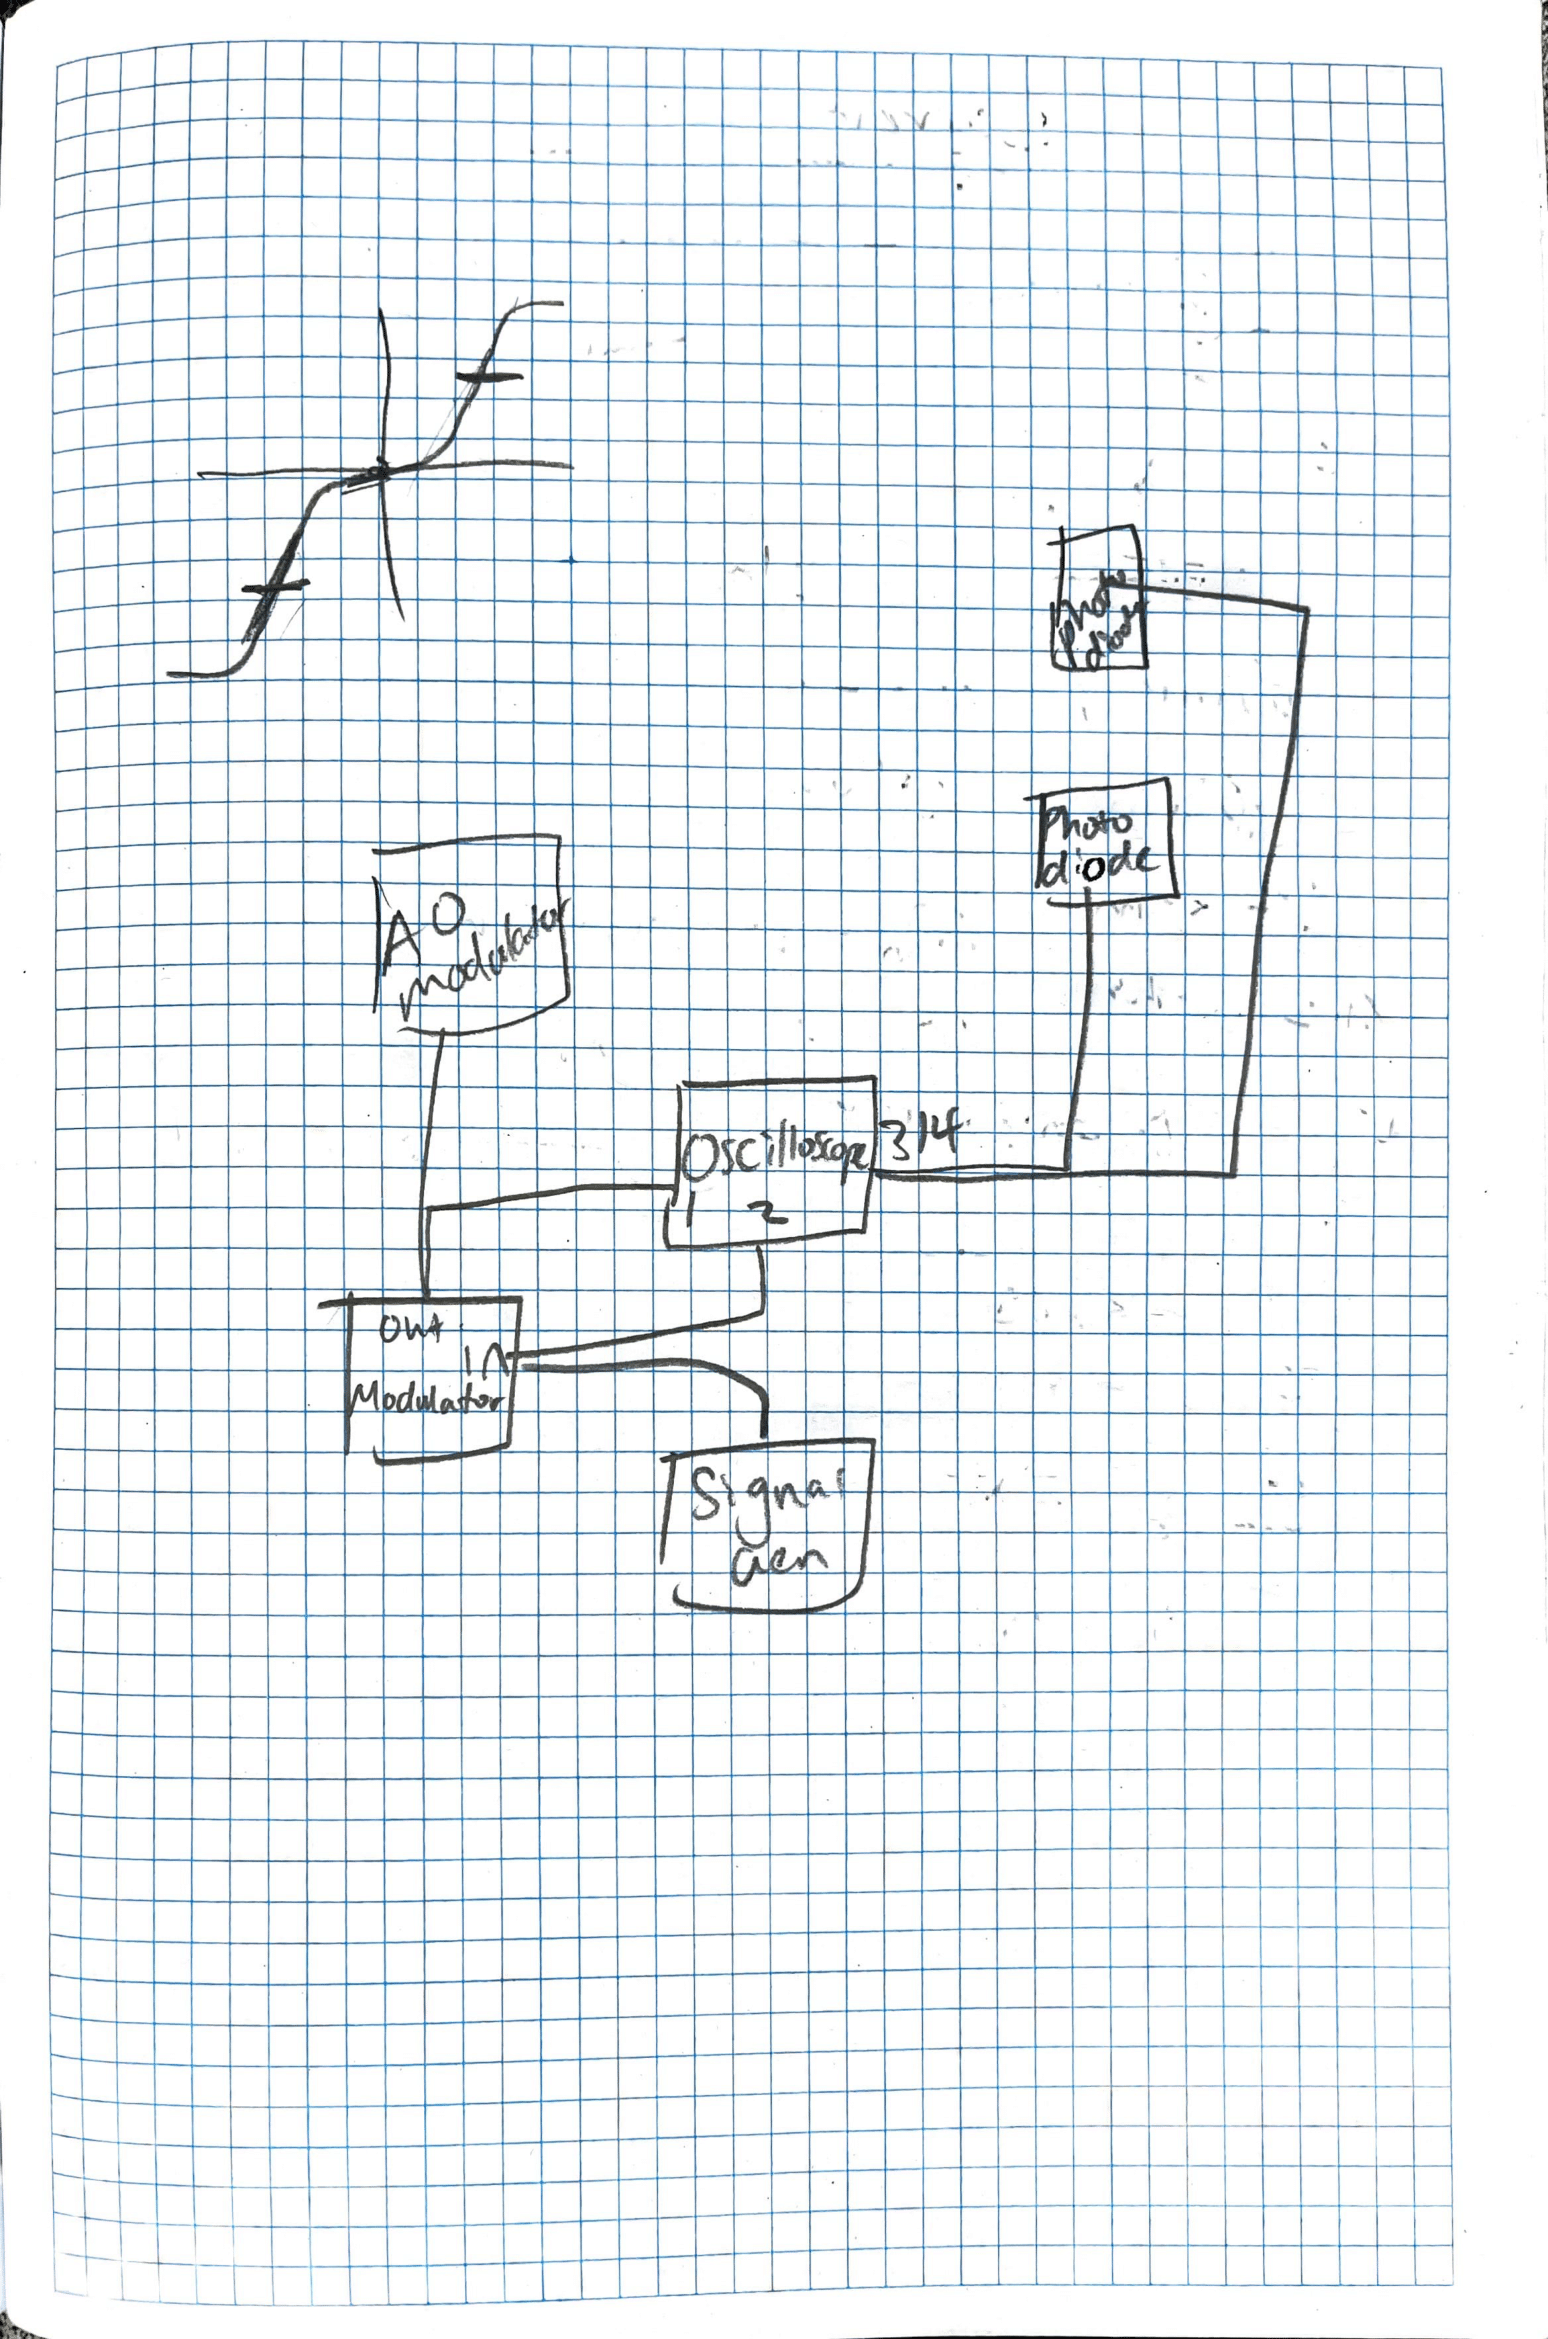
\includegraphics[width=0.3\textwidth]{../Figures/labbook2.png}} \\
    \subfloat[]{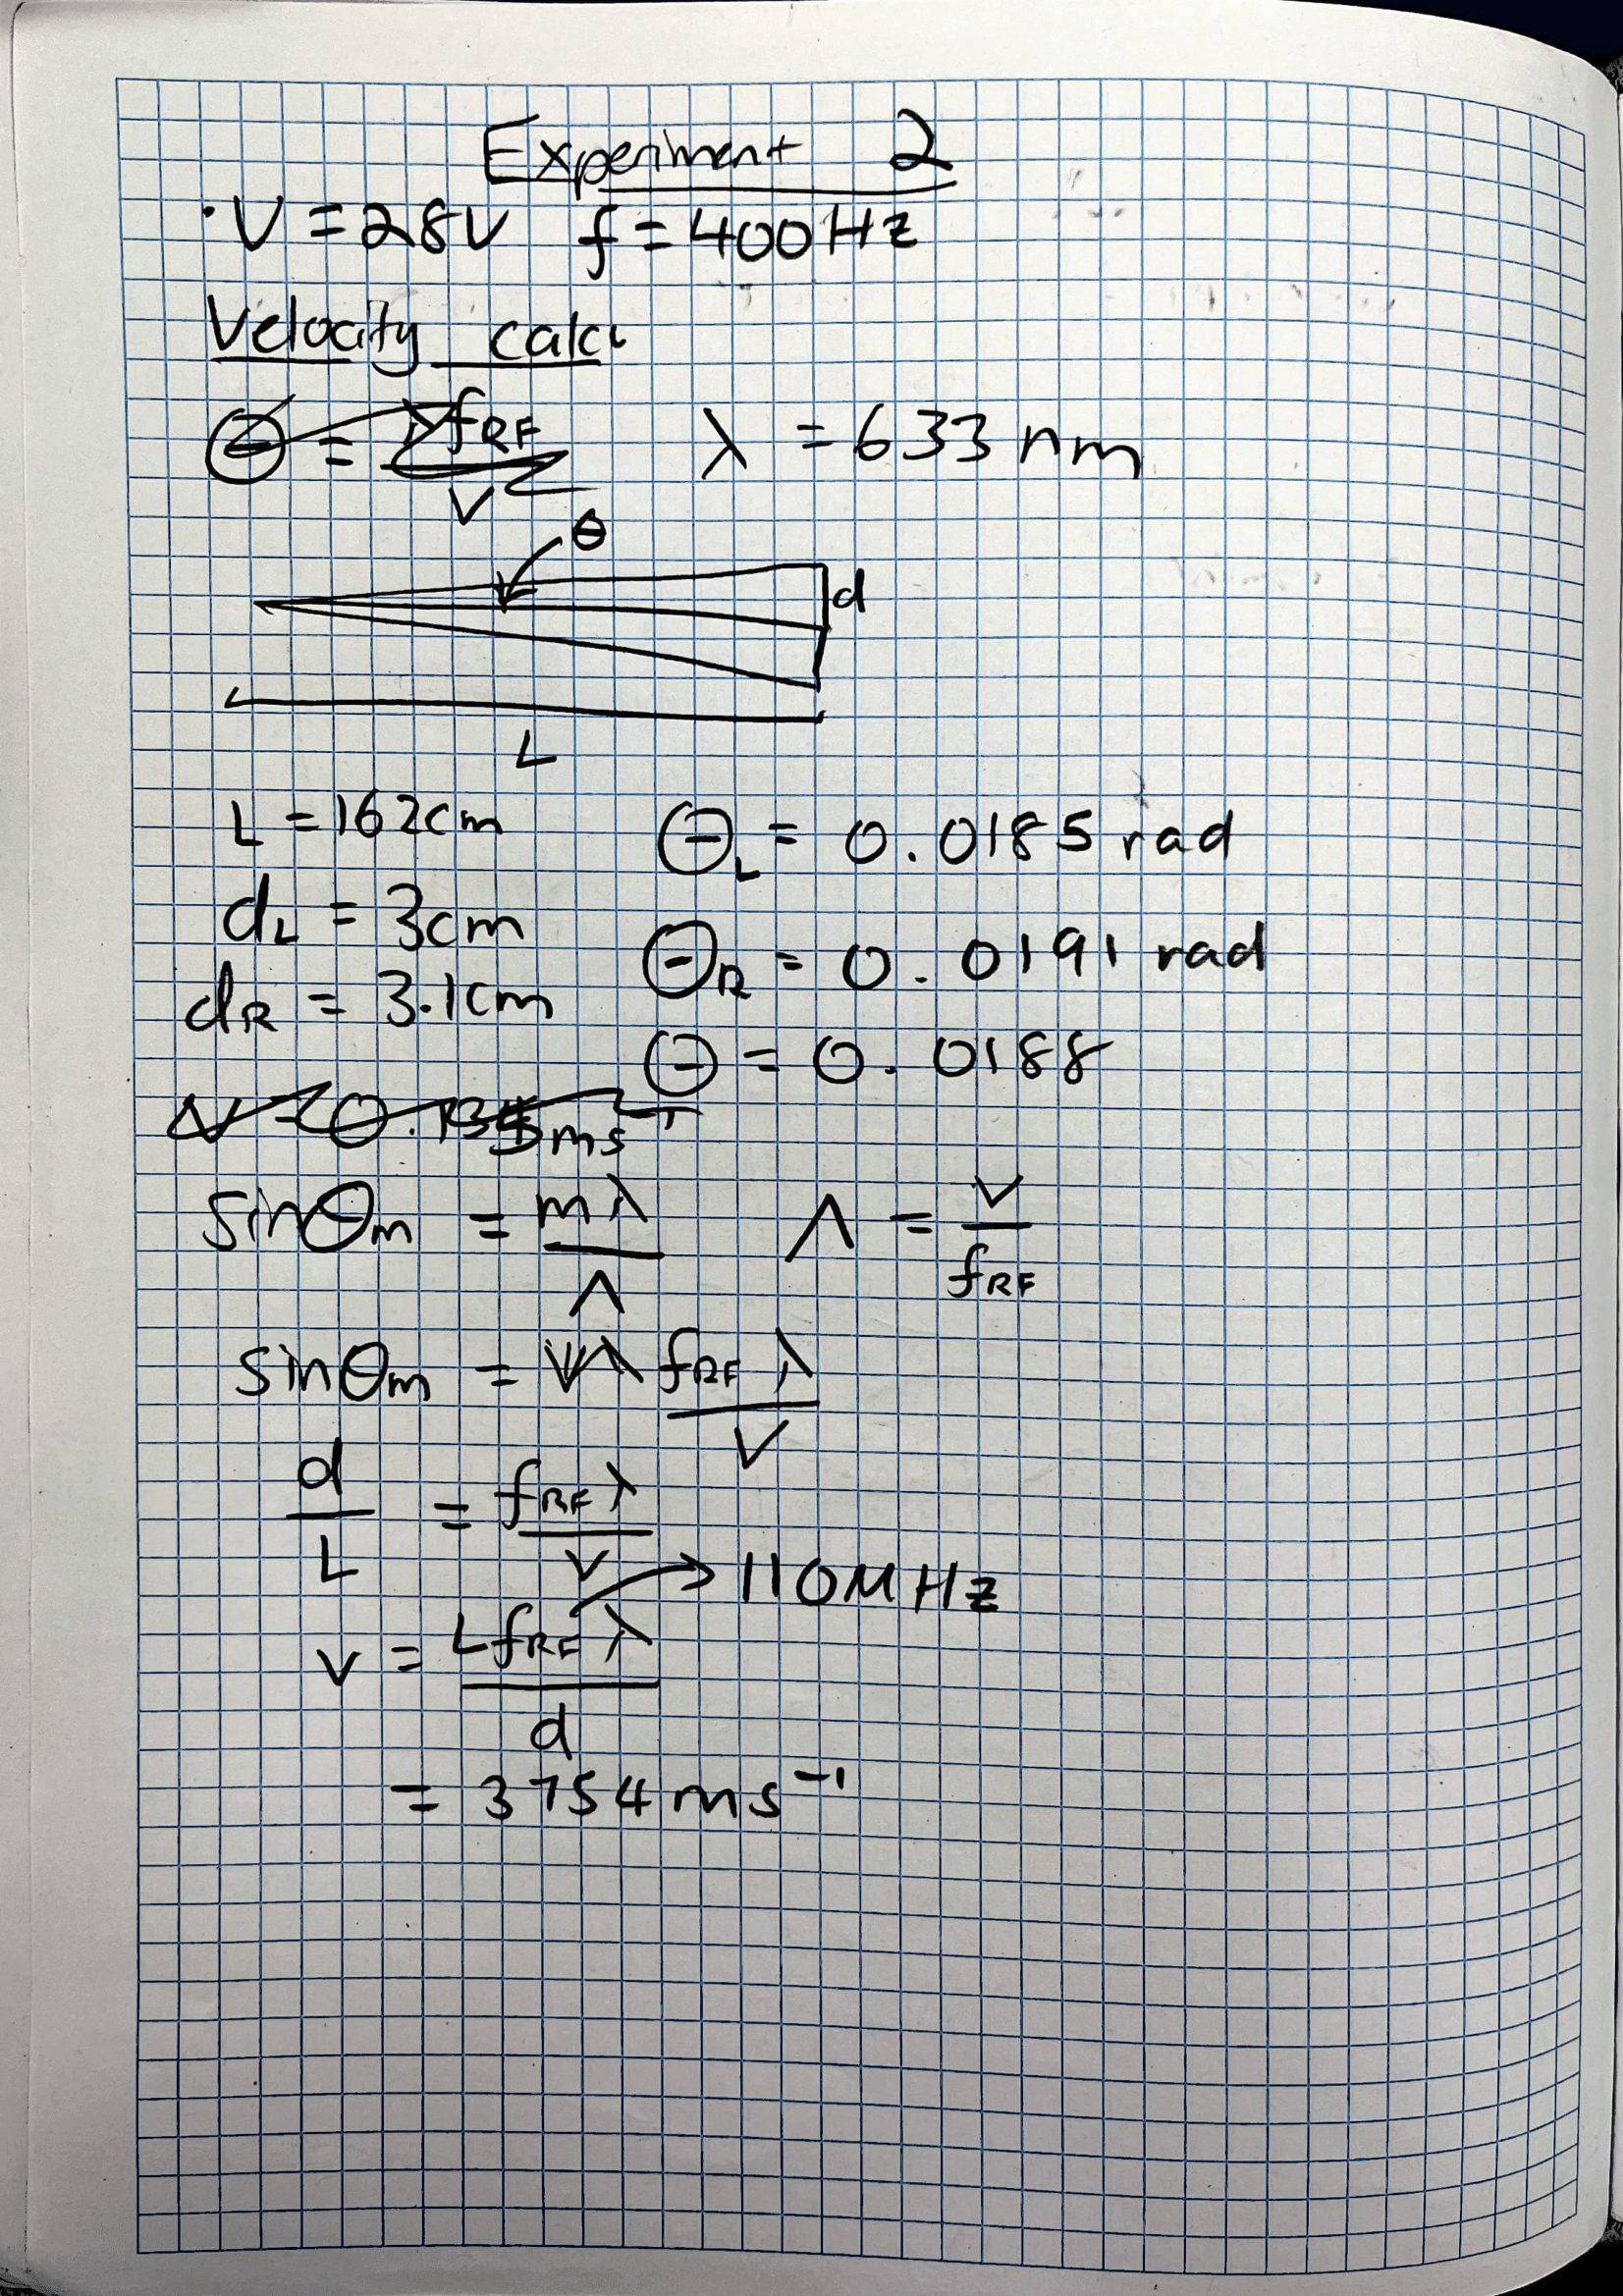
\includegraphics[width=0.3\textwidth]{../Figures/labbook3.png}}
    \subfloat[]{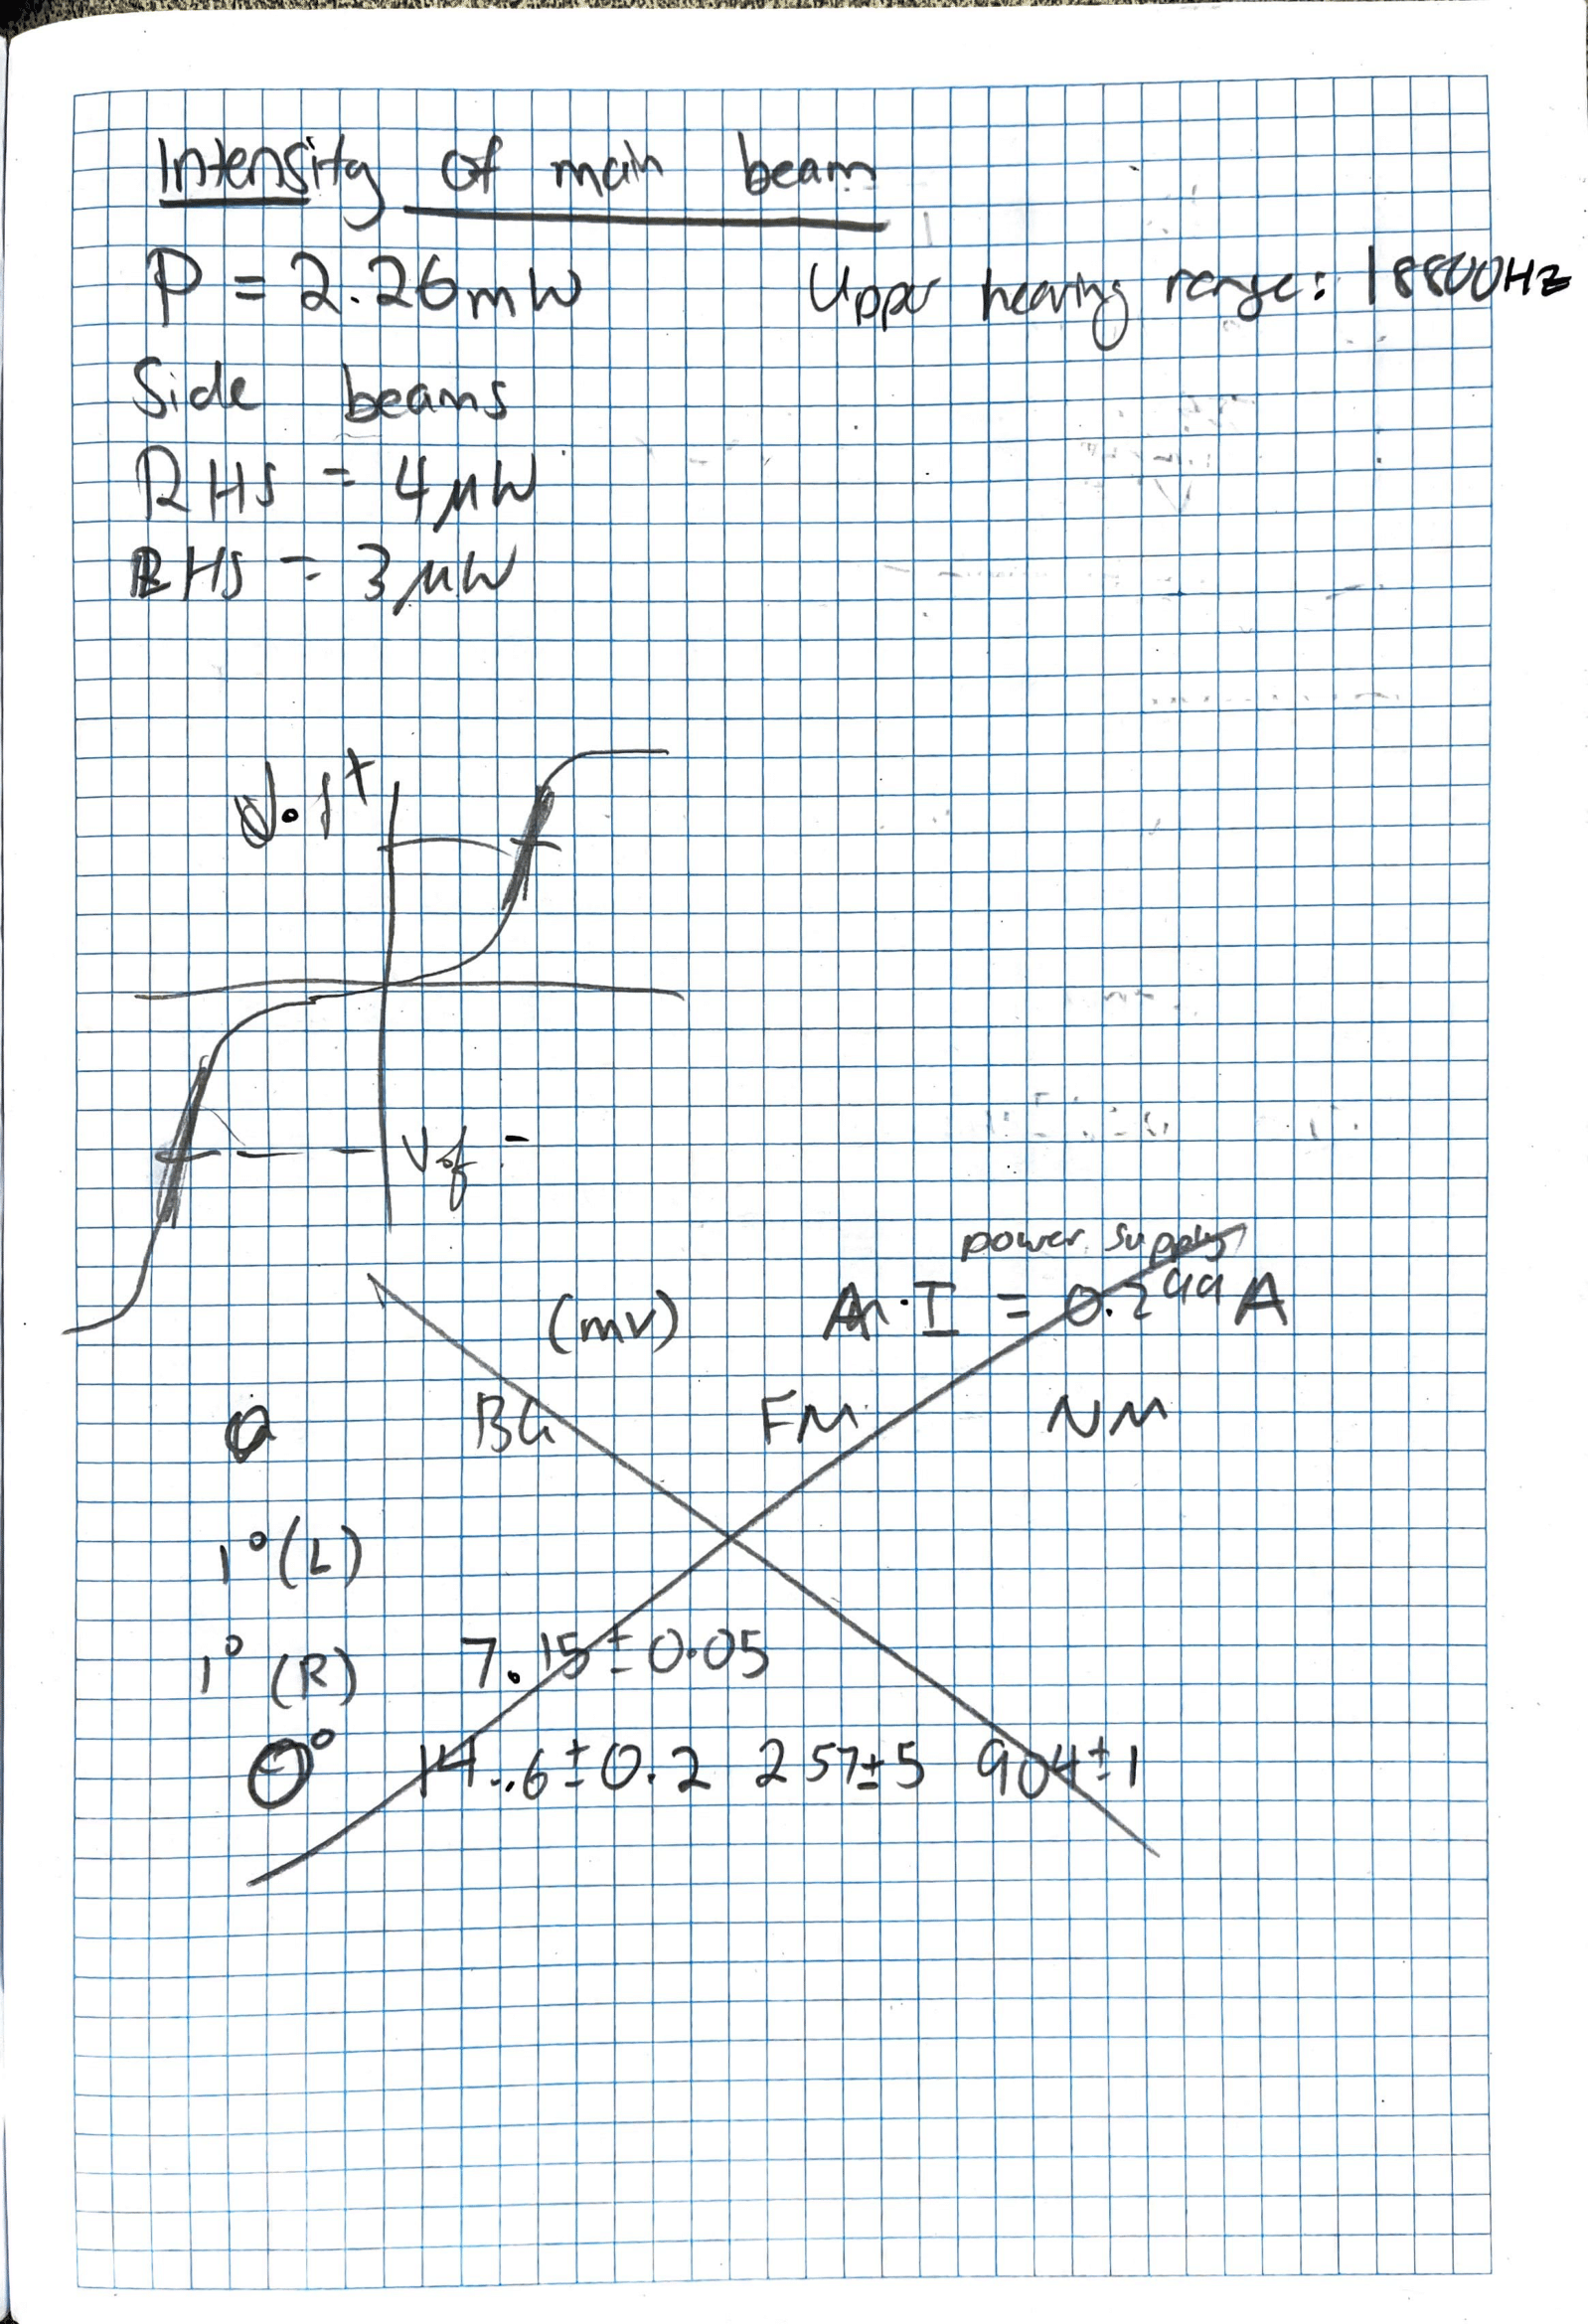
\includegraphics[width=0.3\textwidth]{../Figures/labbook4.png}} \\
    \subfloat[]{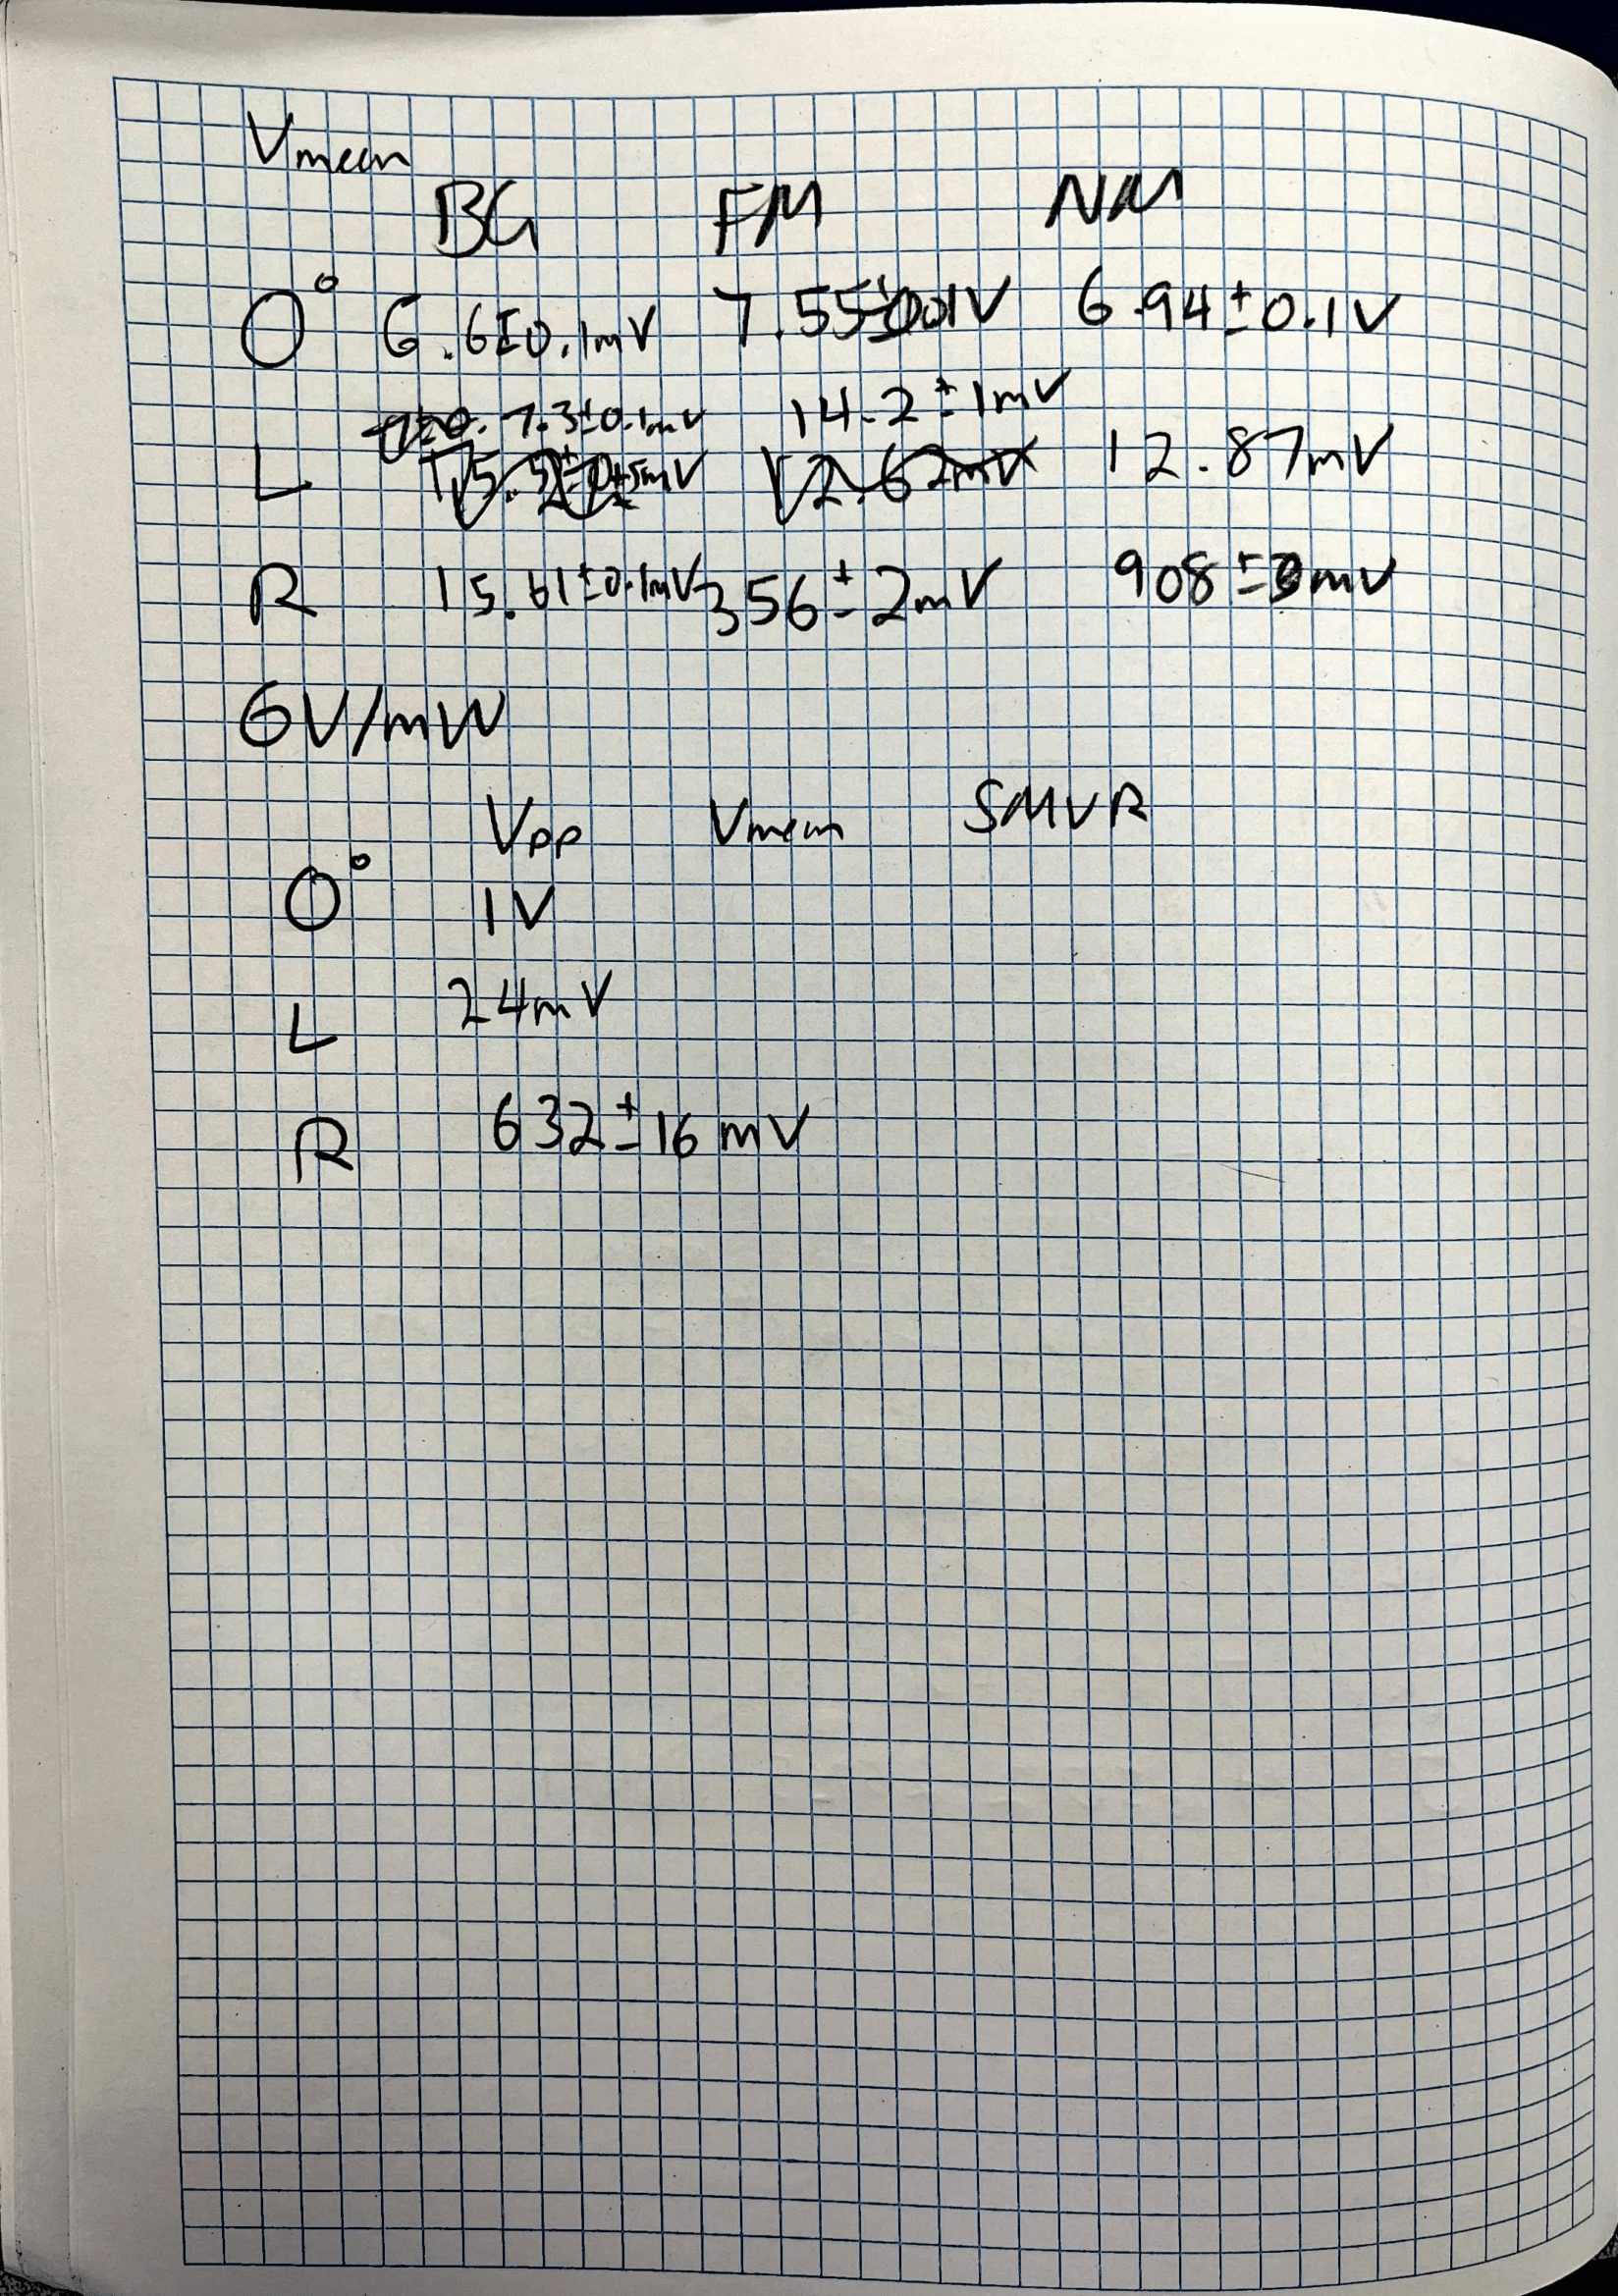
\includegraphics[width=0.3\textwidth]{../Figures/labbook5.png}}
\end{figure*}

\section{Python}
\begin{figure*}[!htbp]
    \begin{python}
    lowmod = pd.read_csv('../Data/lower modulation.csv')
    t = lowmod['ch1_time(s)'] + 0.007
    envelope = lowmod['ch1_value(V)']
    signalgen = lowmod['ch2_value(V)']
    result = lowmod['ch4_value(V)']

    plt.scatter(
        t,
        envelope,
        c='royalblue'
    )

    plt.scatter(
        t,
        result,
        c='darkorange'
    )

    plt.scatter(
        t,
        signalgen,
        c='deeppink'
    )

    plt.xticks([])
    plt.yticks([])

    plt.xlabel('Time')
    plt.ylabel('Power')

    plt.xlim(0,0.005)
    plt.savefig('../Figures/lowmodplot',bbox_inches = 'tight')
    plt.show()
    \end{python}
    \caption{Example code for plotting the figures in Figure \ref{fig:main}.}
\end{figure*}

\begin{figure*}
    \begin{python}
    N = 2**10
    lowmod = pd.read_csv('../Data/lower modulation.csv').sample(N)
    t = lowmod['ch4_time(s)'] + 0.007
    lowmod = lowmod.sort_values(by='ch4_time(s)',ascending=True)
    result = lowmod['ch4_value(V)'] - lowmod['ch4_value(V)'].mean()
    fs = N / (t.max() - t.min())

    window = np.hamming(N)

    fftl = np.fft.rfft(result*window, N)
    fftfreq = np.fft.rfftfreq(N, 1/fs)

    plt.xlim(0,5000)

    plt.xlabel('Frequency (Hz)')
    plt.yticks([])

    power = np.abs(fftl)**2

    peak_index = np.argmax(power)

    peak_freq = fftfreq[peak_index]

    print(f'Peak frequency: {peak_freq:.2f} Hz')

    plt.plot(fftfreq,np.abs(fftl**2),c='royalblue')
    plt.savefig('../Figures/lowmodfourier',bbox_inches = 'tight')
    plt.show()
    \end{python}
    \caption{Example code for plotting the power spectrum. Note the use of 
    the Hamming window. This was chosen over other windows as the Hamming window 
    reduces the effects of sidelobes but retains and accentuates peaks.}
\end{figure*}

\begin{figure*}
    \begin{python}
    power = np.abs(fftl)**2
    fftfreq = np.fft.rfftfreq(N, 1/fs)

    peak_index = np.argmax(power)
    peak_freq = fftfreq[peak_index]
    peak_power = power[peak_index]
    half_max = peak_power / 2

    left_index = peak_index
    while left_index > 0 and power[left_index] > half_max:
        left_index -= 1

    right_index = peak_index
    while right_index < len(power) - 1 and power[right_index] > half_max:
        right_index += 1

    f_left = fftfreq[left_index]
    f_right = fftfreq[right_index]

    fwhm = f_right - f_left

    print(f"Peak frequency: {peak_freq:.2f} Hz")
    print(f"FWHM: {fwhm:.2f} Hz")
    \end{python}
    \caption{Code for finding the full width at half maximum}
\end{figure*}

\begin{figure*}
    \begin{python}
    def bessel(deltaphi, theta_deg, k,offset,width=0.05,acoustic_wavelength=110*10**6):
        theta = np.radians(theta_deg)
        return k*jv(1, deltaphi *1/np.cos(theta) * np.sin(np.pi * width * np.tan(theta)/acoustic_wavelength)/(np.pi*width*np.tan(theta)/acoustic_wavelength)-offset)**2

    def bessel_fit(theta_deg, deltaphi,k,offset):
        return bessel(theta_deg, deltaphi,k,offset)
    \end{python}
    \caption{Code for fitting first order Bessel Function.}
\end{figure*}

\bibliographystyle{apsrev4-2}
\bibliography{../Bibliography/references}

\end{document}
